%!TEX root = THinstituteReport_1.tex

%%%%%%%%%%%%%%%%%%%%%%%%%%%%%%%%%%%%%%%%%
%\section{Analysis of radiation phase space}
\section{Mapping the splittings of in-medium jets}
\label{sec:phasespace}
%%%%%%%%%%%%%%%%%%%%%%%%%%%%%%%%%%%%%%%%%


%%%%%%%%%%%%%%%%%%%%%%%%%%%%%%%%%%%%%%%%%
\subsection{Theoretical considerations}
\label{sec:phasespace-theory}
%%%%%%%%%%%%%%%%%%%%%%%%%%%%%%%%%%%%%%%%%


Jets are multi-particle observables and are experimentally accessed by assembling measured tracks and calorimeter energy deposition, or a combination of both, according to a jet algorithm. In the context of perturbative QCD, multiple splittings inside the jet cone have to be taken into account due to the mass singularity of QCD. 
In the medium, these splittings happen concurrently with, and are affected by, final-state interactions with the surrounding medium. It is therefore worth considering how medium scales, related to the medium size\footnote{For simplicity, in this section we treat the medium as static, where all jets traverse the same length $L$.} and the local properties, will have an impact on the phase space of jet observables. 

%%%%%%%%%%%%%%%%%%%%%%%%%%%%%%%%%%%%%
\begin{figure}
\centering
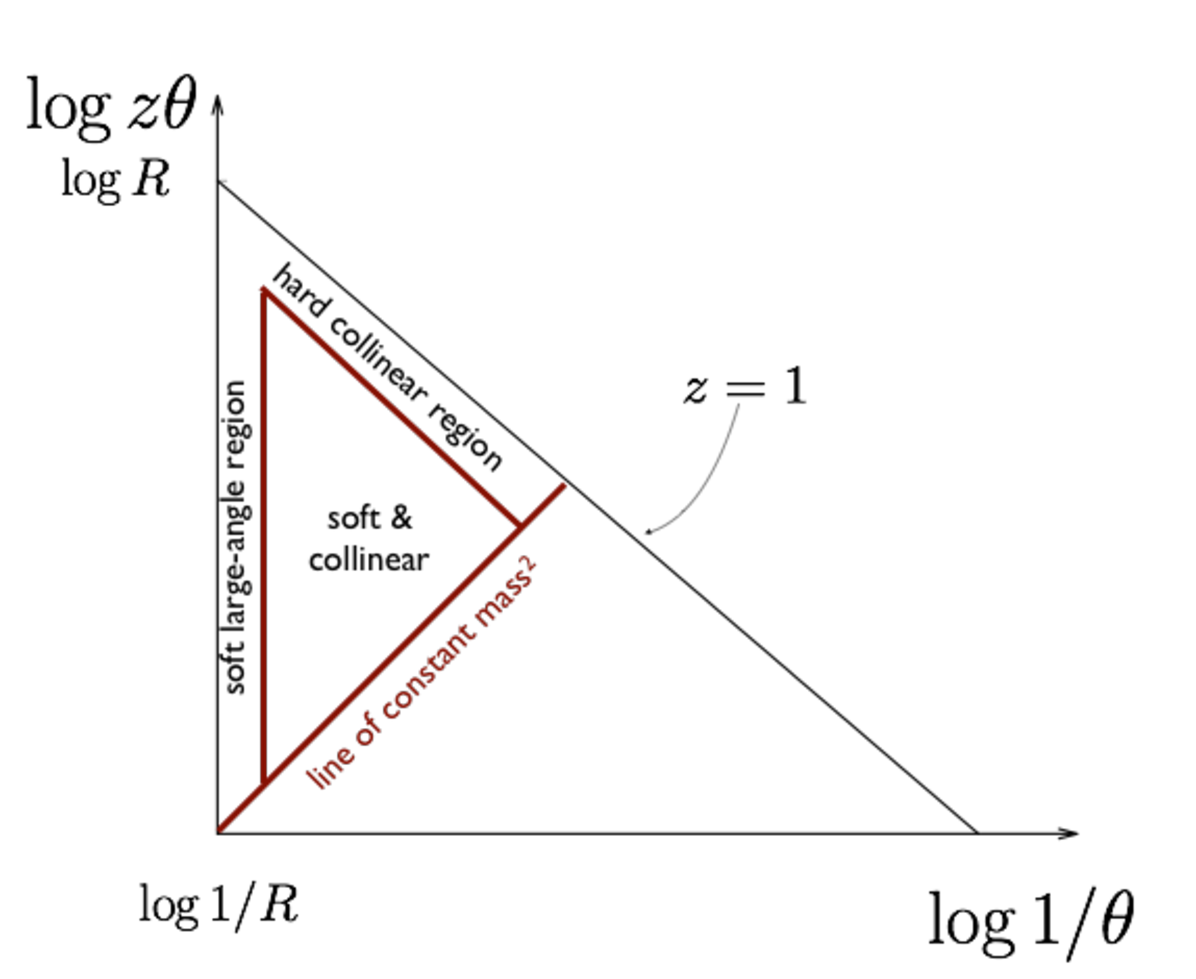
\includegraphics[width=0.6\textwidth]{figures/kinematics/lund_2}%
\caption{Lund kinematical diagram for vacuum radiation. Figure adapted from Ref.~\cite{Dasgupta:2013ihk}.}
\label{fig:PS0}
\end{figure}
%%%%%%%%%%%%%%%%%%%%%%%%%%%%%%%%%%%%%
In this context, it is very useful to introduce the Lund kinematical diagram \cite{Andersson:1988gp} for an arbitrary $1\to 2$ splitting process.
\kmt{Perhaps better do discuss kinematics first, then probability + multiple splittings?}
In the soft and collinear limit, and in the absence of medium interactions, the differential probability $\dd P$ of emission of a gluon is given in terms of its kinematical variables by \cite{Dokshitzer:1991wu,Ellis:1991qj}
\beq
\label{eq:vacuum-phase-space}
\dd P = 2\frac{\alpha_s C_i}{\pi}\, \dd \log z\theta \, \dd \log\frac{1}{\theta} \,,
\eeq
where $z$ and $\theta$ are the energy sharing fraction of and angle between the constituents of a dipole
%the gluon that is emitted off a projectile parton 
in arbitrary color representation ($C_i=C_F$ for quark and $C_i = N_c$ for gluon splitting, respectively). Hence, for fixed coupling, the area spanned below the line $z=1$, see \autoref{fig:PS0}, is uniformly populated by emissions with weight $2\alpha_s C_i/\pi$.
The radiation can take place up to the jet opening angle $R$.
In this figure we have also explicitly mapped out the regimes of soft, large-angle  and hard, collinear radiation. For future reference, it is worth keeping in mind that lines at fixed transverse momentum are horizontal, lines at fixed angle vertical, lines at fixed mass diagonal with a positive unit slope, and lines at fixed energy diagonal with a negative unit slope in this diagram. 
\kmt{What are the axes in the plot we are producing ($\ln\kT/E$ and $\ln R/\theta$)? Where do you hit the non-perturbative regime?}

Before discussing any additional elastic or inelastic processes arising by the presence of a medium, one could consider the fate of vacuum emissions given a certain medium size. It can most naively be compared with the time it takes for a original parton to split into two daughter partons of invariant mass 
\beq
\label{eq:DipoleMass}
%M^2 = z(1-z)\pT^2 \theta^2 \,,
M^2 = z(1-z) E^2 \theta^2 \,,
\eeq
for small angles $\theta$, where $E$ is the total momentum of the dipole
%longitudinal momentum of the parent parton, 
see Eq.~(\ref{eq:vacuum-phase-space}). This time is the so-called \textsl{formation time}, and is related to the uncertainty of the time-scale of splitting $\tform \sim \Delta E^{-1}$, and is explicitly given by
\beq
\label{eq:FormationTime}
%\tform = \frac{2 z(1-z)\pT }{k_\perp^2} = \frac{2 \pT}{M^2} \,,
\tform = \frac{2 z(1-z)E }{\kT^2} = \frac{2 E}{M^2} \,,
%(z \pT \theta^2)^{-1} \,,
\eeq
where 
%$k_\perp = z(1-z)\pT \theta$, in the small angle limit, is the relative transverse momentum of the splitting. 
$\kT = z(1-z) E \theta$ is the (relative) transverse momentum of the dipole in the small angle limit. 
This formula can easily be understood as the time-scale for decaying in the rest frame of the parent times its boost factor $\sim (1/M) \times (E/M)$. In the following, we will only consider soft radiation and neglect additional numerical factors to write $\tform \sim (z E \theta^2)^{-1} $.

Coming back to the diagram, let us identify emissions that happened inside the medium or, in other words, formation times that are shorter than the medium length ($\tform < L$). 
This condition results in an area on the Lund diagram delimited by the line solving $\tform = L$,
\beq
\log z \theta = \log \frac{1}{\theta} + \log \frac{1}{\pT L} \,,
\eeq
which is also represented in \autoref{fig:PS1}. Hence, the area above the line marked $\tform = L$ correspond to (vacuum) emissions that occur inside the medium. Emissions with $\tform > L$ occupy the region below the line.

In order to proceed, we will have to assume something about how the jet constituents interact with the medium. For illustrative purposes we will assume that all propagating particles experience diffusive momentum broadening, where the amount of accumulated momentum is characterized by the dispersion $\langle \kT^2 \rangle = \hat q t$, $t$ determining the time of in-medium propagation. The jet transport coefficient $\hat q$ acts as a diffusion constant in transverse space for the hard modes.\footnote{In this discussion, we neglect the influence of rare, hard kicks in the medium that go beyond this definition.} 
%While this reflects the expectation from multiple, soft interaction with a plasma and neglects rare, hard collisions, the latter can easily be incorporated into the same discussion.

%%%%%%%%%%%%%%%%%%%%%%%%%%%%%%%%%%%%%
\begin{figure}
\centering
%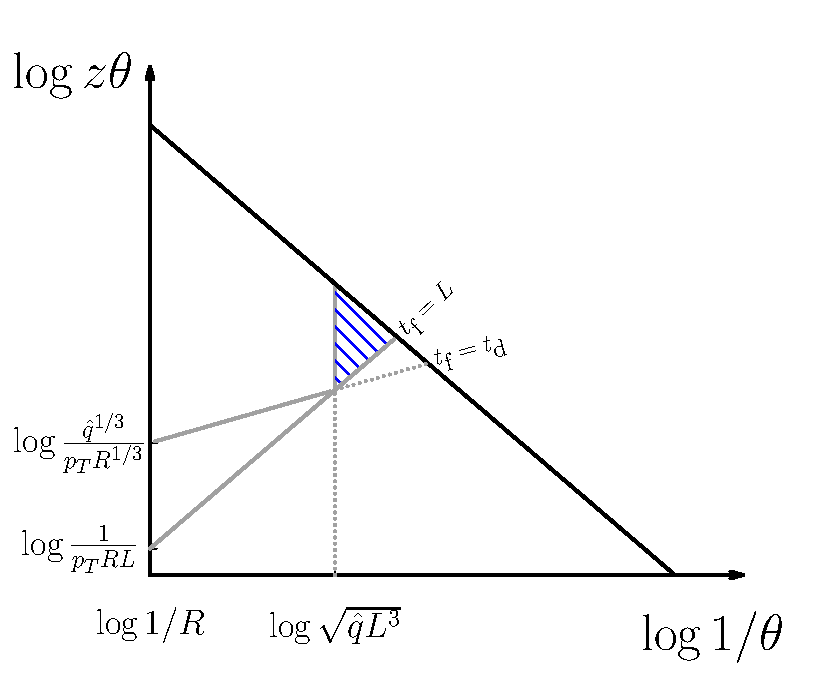
\includegraphics[width=0.5\textwidth]{figures/kinematics/plotVac}%
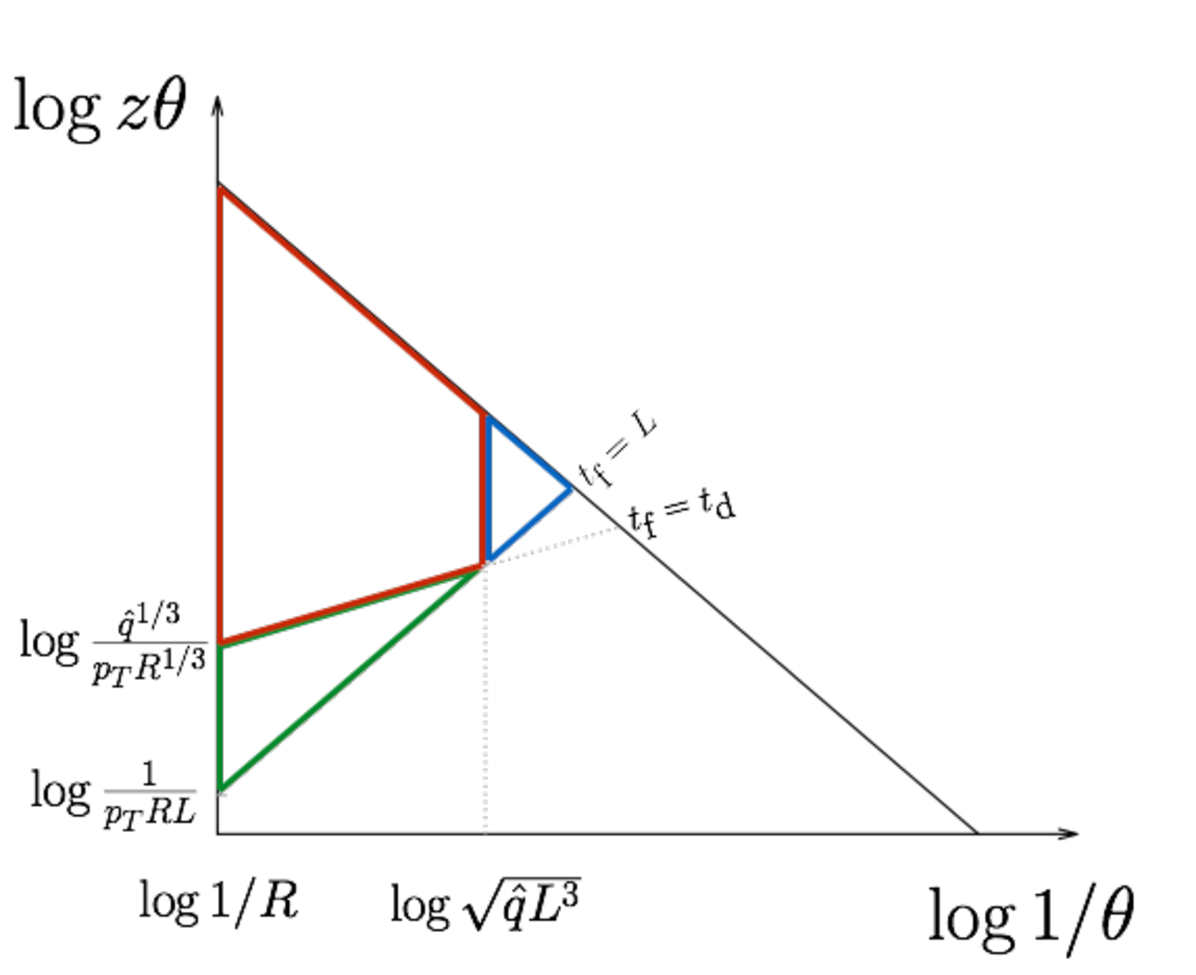
\includegraphics[width=0.6\textwidth]{figures/kinematics/lund_regions_colored}%
%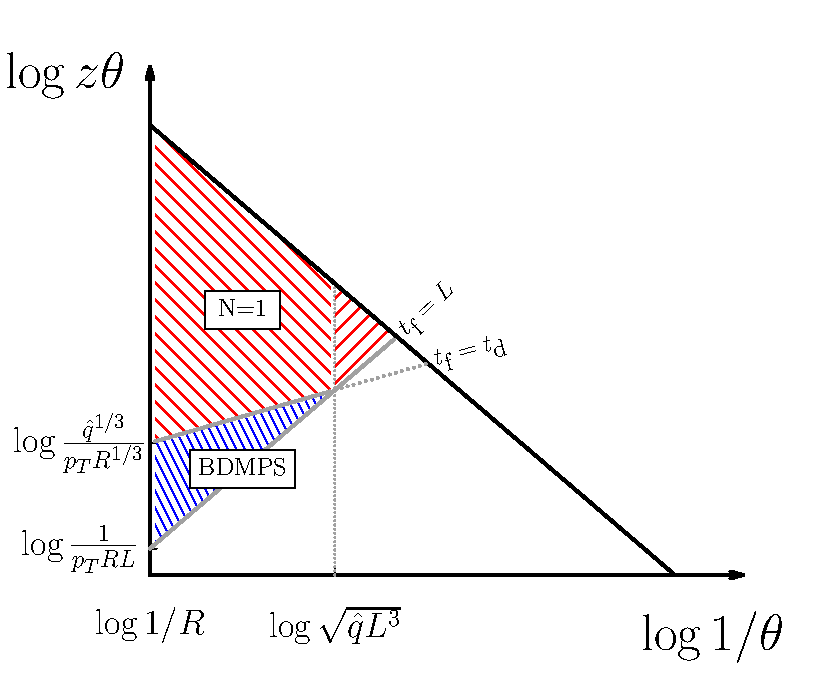
\includegraphics[width=0.5\textwidth]{figures/kinematics/plotMed}
\caption{Lund diagram for vacuum radiation with inclusion of relevant medium scales related to creation and decoherence of partons in the medium. The parameters are $\hat q = $ 2 GeV$^2$/fm, L = 2 fm and $p_{\scriptscriptstyle T}$ = 300 GeV. 
%Right: Lund diagram for medium induced radiation.
}
\label{fig:PS1}
\end{figure}
%%%%%%%%%%%%%%%%%%%%%%%%%%%%%%%%%%%%%
Having this picture in mind, a second time-scale immediately becomes relevant. It is typically referred to as the decoherence time, since it gauges whether medium interactions resolve a particular splitting. This occurs whenever the size of the pair, which can be estimated as $x_\perp \sim \theta t$ for small angles, becomes comparable to the medium resolution scale $\lambda_\perp \sim(\hat q t)^{-\onehalf}$ which in turn is inverse to the transverse momentum accumulated by multiple scattering.
By equating the two, $x_\perp \sim \lambda_\perp$, we find the parametric estimate for the resolution time which turns out to be
\beq
\label{eq:DecoherenceTime}
\tdecoh = \left( \hat q \theta^2 \right)^{-\onethird} \,,
\eeq
which corresponds to the time scale where the dipole constituents decorrelate in color space.
Hence the line $\tform = \tdecoh$ is parameterized by
\beq
\log z\theta = \frac{1}{3} \log \frac{1}{\theta} + \log \frac{\hat q ^\onethird}{\pT} \,,
\eeq
and the area above this line represents the phase space for vacuum emissions.
As is clear from \autoref{fig:PS1}, this guarantees that at angles smaller than the minimal decoherence angle $\theta_c \sim (\hat q L^3)^{-\onehalf}$, the decoherence time is automatically larger than the medium length.\footnote{Since, $\tdecoh >L$ doesn't make much sense physically, we have represented this element by a dashed line in \autoref{fig:PS1}.} In particular, emissions with $\tform< \tdecoh < L$ correspond to pure vacuum splittings inside the medium that, during their subsequent propagation and possible further branching, will be resolved by medium interactions. Note also that the intersection point $\tform = \tdecoh$ corresponds to emissions with a transverse momentum scale $Q_s \sim(\hat q L)^{1/2}$ and the characteristic energy $\omega_c \sim \hat q L^2$.
The three time-scales we have identified -- the formation time, $\tform$, the decoherence time, $\tdecoh$, and the length of the medium, $L$ -- can be arranged in three possible orderings. These are marked out on \autoref{fig:PS1} as $\tform < \tdecoh < L $ by the red area, $\tform < L < \tdecoh$ by the blue area and $\tdecoh < \tform < L$ by the green area, respectively. 
%{\it The phase space of these regions is given by their area, and is easily found to be
%\begin{align}
%{\color{red} A_{\tform < \tdecoh < L}} &{\color{red}= \frac{1}{2}\ln \frac{R^2}{\theta_c^2} \left(\ln \frac{\pT}{\omega_c} + \frac{1}{3}\ln \frac{R^2}{\theta_c^2} \right)}  \,,\\
%{\color{blue} A_{\tform < L < \tdecoh}} &{\color{blue}= \frac{1}{4} \ln^2 \frac{\pT}{\omega_c}} \,,\\
%{\color{OliveGreen} A_{\tdecoh < \tform < L}} &{\color{OliveGreen}= \frac{1}{12} \ln^2 \frac{R^2}{\theta_c^2}} \,,
%\end{align}
%for $\pT > \omega_c$, where $\omega_c = \hat q L^2$.
%It is worth pointing out, that vacuum emissions that are emitted inside the medium at sufficiently small angles, $\theta < \theta_c$, remain unresolved by interactions with the medium \cite{MehtarTani:2010ma,MehtarTani:2011tz}. This implies that splittings in this region should follow a vacuum emission pattern, yet the jet is quenched (coherently) due to the presence of a total color charge \cite{CasalderreySolana:2012ef}. }
%It poses an exciting  challenge to pin this region down experimentally.
The second ordering is particularly interesting, giving rise to splittings that are formed inside the medium yet remain completely unresolved by medium interactions due to strong interference effects. It is often referred to as the coherence regime.

Before moving on, let us briefly contemplate a different mechanism of medium interactions based on incoherent scatterings.
%model for the medium interactions.
In this case, the resolution scale of the medium is simply the inverse of the medium momentum exchange, $\lambda_\perp \sim q_\perp^{-1}$. Now, the decoherence time is $\tdecoh \sim (\theta q_\perp)^{-1}$ which gives to a minimal coherence angle $\theta_c \sim (q_\perp L)^{-1}$. In effect, the coherence regime exists only for sufficiently soft interactions $q_\perp < \sqrt{\pT/L}$.

Now let us briefly review the possible additional radiative channels that are opened due to interactions with the medium. It is important to stress that the emission probability for medium-induced radiation, such as Eq.~(\ref{eq:vacuum-phase-space}) for the vacuum radiation, does not factorize in the same way. Hence, the phase space in the Lund diagram is not anymore uniformly filled. 

Let us firstly describe the multiple scattering regime. It applies to situations when, in course of their formation, induced gluons experience transverse momentum broadening, approximated by $\langle k_\perp^2 \rangle \lesssim \hat q \tform$, see e.g. \cite{Kurkela:2014tla} for a more thorough discussion. We can invert this relation to find that the formation time of the emitted particles becomes $\tform(\omega) \sim \sqrt{\omega/\hat q}$. 
Gluons with the longest formation time $\tform= L$, carry energy $\omega_c \sim \hat q L^2$.
%Reciprocally, $k_{\rm f}^2 \sim \sqrt{\hat q \omega}$ or, in terms of emission angle, $\theta_{\rm f}(\omega) \sim (\hat q/\omega^3)^{\onefourth}$. 
%The spectrum of emitted gluons per unit of energy is therefore
%\beq
%\label{eq:BDMPS-spectrum}
%\dd {\cal P}_{\rm med} = 2 \frac{\alpha_s C_{\tiny R}}{\pi} \frac{L}{\tform(\omega)}\frac{\dd \omega}{\omega} \,,
%\eeq
%for $\tform \ll L$ or, in other words, $\omega \ll \omega_c$, where $\omega_c \sim \hat q L^2$. 
This energy scale also acts as an effective cut-off scale, as for $\omega > \omega_c$ the spectrum is strongly suppressed (LPM suppression). It also determines a ``minimal'' angle for gluon emission due to multiple scattering, denoted $\theta_{\rm f}(\omega_c) \sim (\hat q L^3)^{-\onehalf}$, that we already encountered as a minimal angle for coherence in the discussion above.
%Hence, LPM radiation contributes maximally along the line $\tform \sim \tdecoh$. 
It involves formation times longer than the decoherence time $\tform \gtrsim \tdecoh$, which implies $k_{\rm f} \lesssim \sqrt{\hat q \omega}$, and angles $\theta > \theta_c$. Furthermore, the multiplicity of LPM gluons becomes large in the soft sector, in particular at $\omega \lesssim \alpha_s^2 \omega_c$. In this regime, resummation of multiple medium-induced gluons is necessary.

This medium-induced radiative component is expected to enhance the yield around $\tform \sim \tdecoh$. It is however worth keeping in mind that due to broadening and subsequent splitting, it is expected that these quanta will be effectively transported out of the jet cone. What remains is therefore a residual impact of ``energy loss'' that affects the vacuum like branchings inside the medium, see \autoref{sec:phasespace-mc} for results from in-medium Monte Carlo showers.

In addition to the (relatively) soft emissions that are sensitive to multiple scattering, there arises a radiative component from rare, hard kicks in the medium. This component is formally higher-twist, i.e. scales as $\sim k_\perp^{-4}$, and has to be induced inside the medium, $\tform < L$. It is however subleading to the the LPM emissions that dominate close to the line $\tform \sim \tdecoh$.
These emissions will typically not undergo further splittings and can contribute to the intra-jet distribution. 

To summarize, from perturbative arguments regarding medium-induced radiative processes we expect to observe large medium-effects in the region marked by green in \autoref{fig:PS1}, which overlaps with the region where LPM radiation is abundant. In the absence of medium interactions, the theoretical expectation is approximately reproduced by vacuum Monte Carlo showers, see \autoref{sec:iterative-declustering} for more details. In \autoref{sec:phasespace-mc} we compare our theoretical expectation with models that implement medium modifications. This concludes the physics discussion of possible radiative contributions at the level of single splitting. It is worth keeping in mind that what we have discussed so far is an idealized picture that will be complicated by the embedding the jets into correlated and un-correlated medium backgrounds. We have also neglected a set of other effects, such as medium back-reaction, that could possibly become important for realistic modeling of the jet-medium interactions. \kmt{Better wording, for further discussion see also Aleksi and Urs.}

\kmt{How to generalize to many splittings? How to connect this section to the rest? In principle, the main effect in the map is running of $\alpha_s$. A secondary (higher-order) effect comes from accumulating soft radiation, contribution scales as $\alpha_s\times$(log-phase space of father).}

%%%%%%%%%%%%%%%%%%%%%%%%%%%%%%%%%%%%%%%%
\subsection{Filling the map from reclustered of jets}
\label{sec:iterative-declustering}
%%%%%%%%%%%%%%%%%%%%%%%%%%%%%%%%%%%%%%%%

The generalization of this picture to multiple emissions is more delicate. In vacuum, subsequent emissions are self-similar (apart from the running of $\alpha_s$) which allows to iterate the splitting process with the jet opening angle R replaced by the splitting angle of the parent dipole (angular ordering) \cite{Dokshitzer:1991wu}. 

In order to connect theory with experimental observables, one relies on an operational definition of what a jet is. Such procedures cluster the final-state stable particles using sequential recombination algorithms, e.g. as implemented in FastJet \cite{Cacciari:2005hq,Cacciari:2011ma}. Final state particles $i$ and $j$ are assigned a mutual distance $d_{ij}$ and a distance to the beam $d_{i\rm B}$. The pair with the smallest distance are recombined first, and the algorithm repeats until the distance to the beam is the smallest quantity. In this case, the algorithm terminates labelling $i$ a jet. The distance metric is generally defined as
\begin{align}
\label{eq:JetDistanceMetric}
d_{ij} &= \min\left(p_{{\rm \tiny T},i}^{2\alpha},p_{{\rm \tiny T},j}^{2\alpha} \right) \frac{\Delta R_{ij}^2}{R^2} \,, \\
d_{i \rm B} &= p_{{\rm \tiny T},i}^{2\alpha} \,,
\end{align}
where $\Delta R_{ij}^2 = (\Delta \phi_{ij})^2 + (\Delta \eta_{ij})^2$ and $\alpha$ is a constant that defines the algortihm; $\Delta \phi_{ij}$ ($\Delta \eta_{ij}$) being the separation of the particles in azimuthal angle (pseudorapidity). In our studies, we have used the anti-$k_{\rm \tiny T}$ algorithm ($\alpha = -1$) \cite{Cacciari:2008gp}, the Cambridge/Aachen (C/A) algorithm ($\alpha = 0$) \cite{Dokshitzer:1997in,Wobisch:1998wt}, and the $k_{\rm \tiny T}$ algorithm ($\alpha = 1$) \cite{Catani:1993hr,Ellis:1993tq}.

Given a reconstructed jet, obtained from a full heavy-ion event, with a list of constituents belonging to it
%, or perhaps after including a stage of additional mitigation of unwanted background, 
one can repeat the recombination using one of the algorithms described above. 
\kmt{There are some known issues in doing this, C/A was originally introduced as an improvement over $k_{\rm \tiny T}$ (note that the azimuthal angle will play a funny role in $\kT$!)\cite{Dokshitzer:1997in} and anti-$k_{\rm \tiny T}$ is usually warned against, see \cite{Salam:2009jx}. We should also refer to Salam, Soyez and Dreyer, in preparation. The more ``reasonable'' way of doing it is build up the Lund plane using C/A and later ``scan'' the plan along different lines... These issues are a reflection of what happens in Fig.~3 - instead of a $\sim$uniformly filled phase space, we see that regions are ``eating up'' contributions from other regions. These issues also show up in the grooming plot which points to some of the pathological properties of (anti-)$k_{\rm \tiny T}$ algorithms. While these issues are mostly coming up in the context of vacuum showering, similar effects are already appearing in QED and will become even worse (?) for no ordered quanta?}
In this context, this is referred to as a reclustering of the jet, providing a complete hierarchical tree (aka ``history'') of the jet evolution. Substructure techniques, to be used extensively throughout this report, define observables based on the information organized in such a tree. 
%Usually, one retraces the nodes of the tree in a stepwise fashion, in a process called declustering.
It is important to keep in mind that, depending on the reclustering algorithm, the information stored in the tree is only approximately related to the sequence of quark and gluon splittings that build the jet structure as understood within perturbative QCD. 
%In vacuum, the correspondence is most reliable for the C/A algorithm due to angular odering, but for medium showers, which comprise particles that are not angular ordered, other algorithms could potentially become relevant.

In order to extract relevant information from a sample of real (simulated) jets, we apply the following procedure.
%Uncovering this sequence of splittings should be in close correspondence to filling the Lund diagram using the following procedure. 
For a given jet in the sample, fill the Lund diagram by
\begin{description}
\item[1)] build a history of splittings by reclustering a jet with a given reclustering algorithm,
\item[2)] at each branching, extract the variables $z$ and $\theta$. Here, we define $z \equiv z_\text{rel} = p_{t,j_2}/(p_{t,j_1}+p_{t,j_2})$ and use $\log(z \Delta R_{j_1 j_2}/R)$ as the quantity on the $y$-axis, where $j_i$ ($i=1,2$) refer to two branches of the tree.
%\footnote{We thank G.~Salam for a discussion on this point.} 
This definition of $z$ has the property that it always reflects the momentum sharing within that  specific step.

\end{description}
%The Lund plane is thus populated for a sample of jets.
The C/A reclustering, where the distance metric is only determined by the angular separation, see Eq.~(\ref{eq:JetDistanceMetric}), should correspond most closely to a angular-ordered sequence of splittings based on our arguments above. That means that the last step of jet reclustering merges two substructures separated at large angles.
Alternative reclustering strategies can however be used, although it would distort the correspondence with showers that implement angular ordering. Given that we also will study other types of parton (or dipole) showers, e.g. that include medium effects, we have also studied the use of the (anti-)$k_{\rm \tiny T}$ algorithms in this step. 
%The strategy of the clustering algorithm manifests itself in the declustering and grooming. CA algorithm combines the closest particles first. As a consequence, the first declustering steps will encounter soft splittings at large angle. 
In the case of the $k_{\rm \tiny T}$-algorithm, the softest particles are clustered first. As a consequence, the last reclustering step will merge hard splittings. The anti-$k_{\rm \tiny T}$ clusters hard particles first, thus splittings at the last reclustering steps will be generally soft. 
%Such ordering is reflected in the Lund plots of \autoref{fig:AlgoDependence}.


%%%%%%%%%%%%%%%%%%%%%%%%%%%%%%%%%%%%%
\begin{figure}[t!]
\centering
%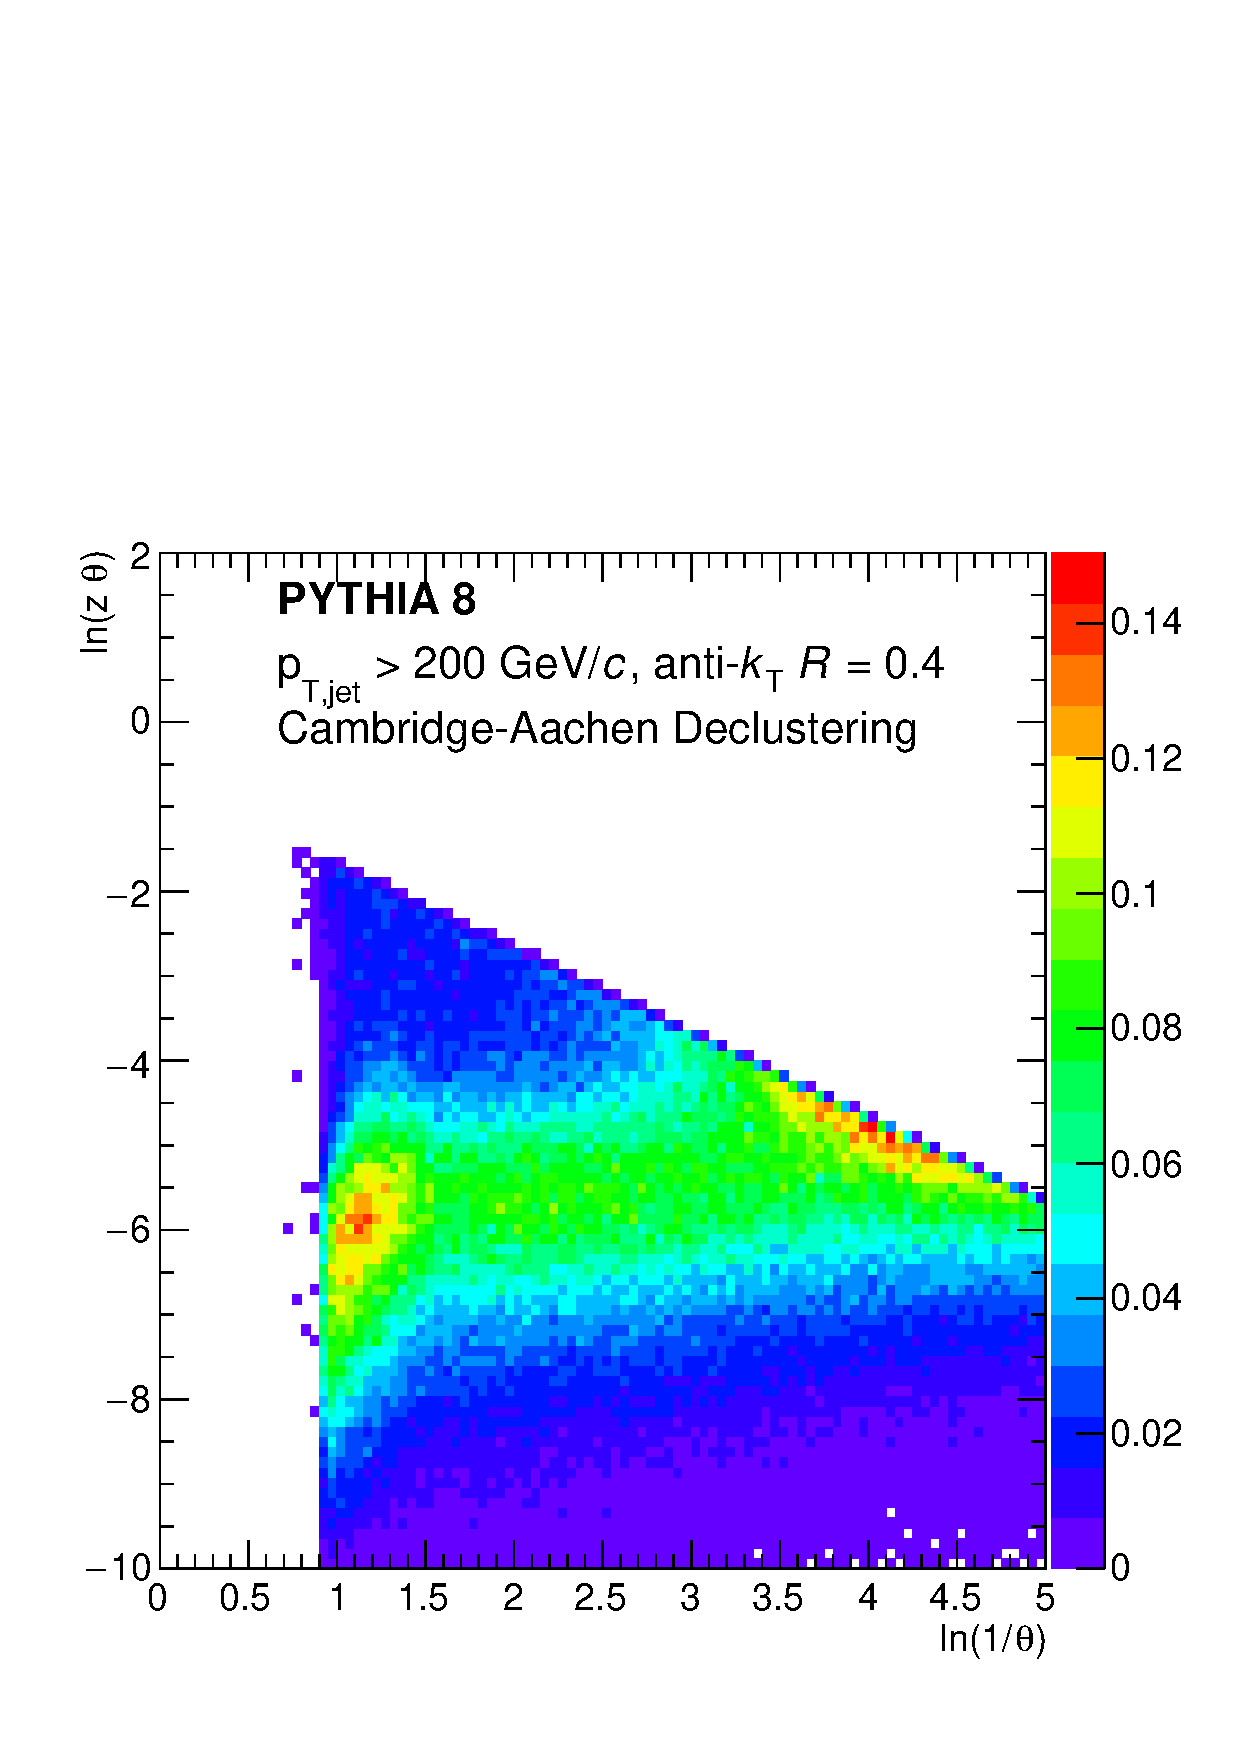
\includegraphics[width=0.33\textwidth]{figures/LundMC/Pythia_CA}
%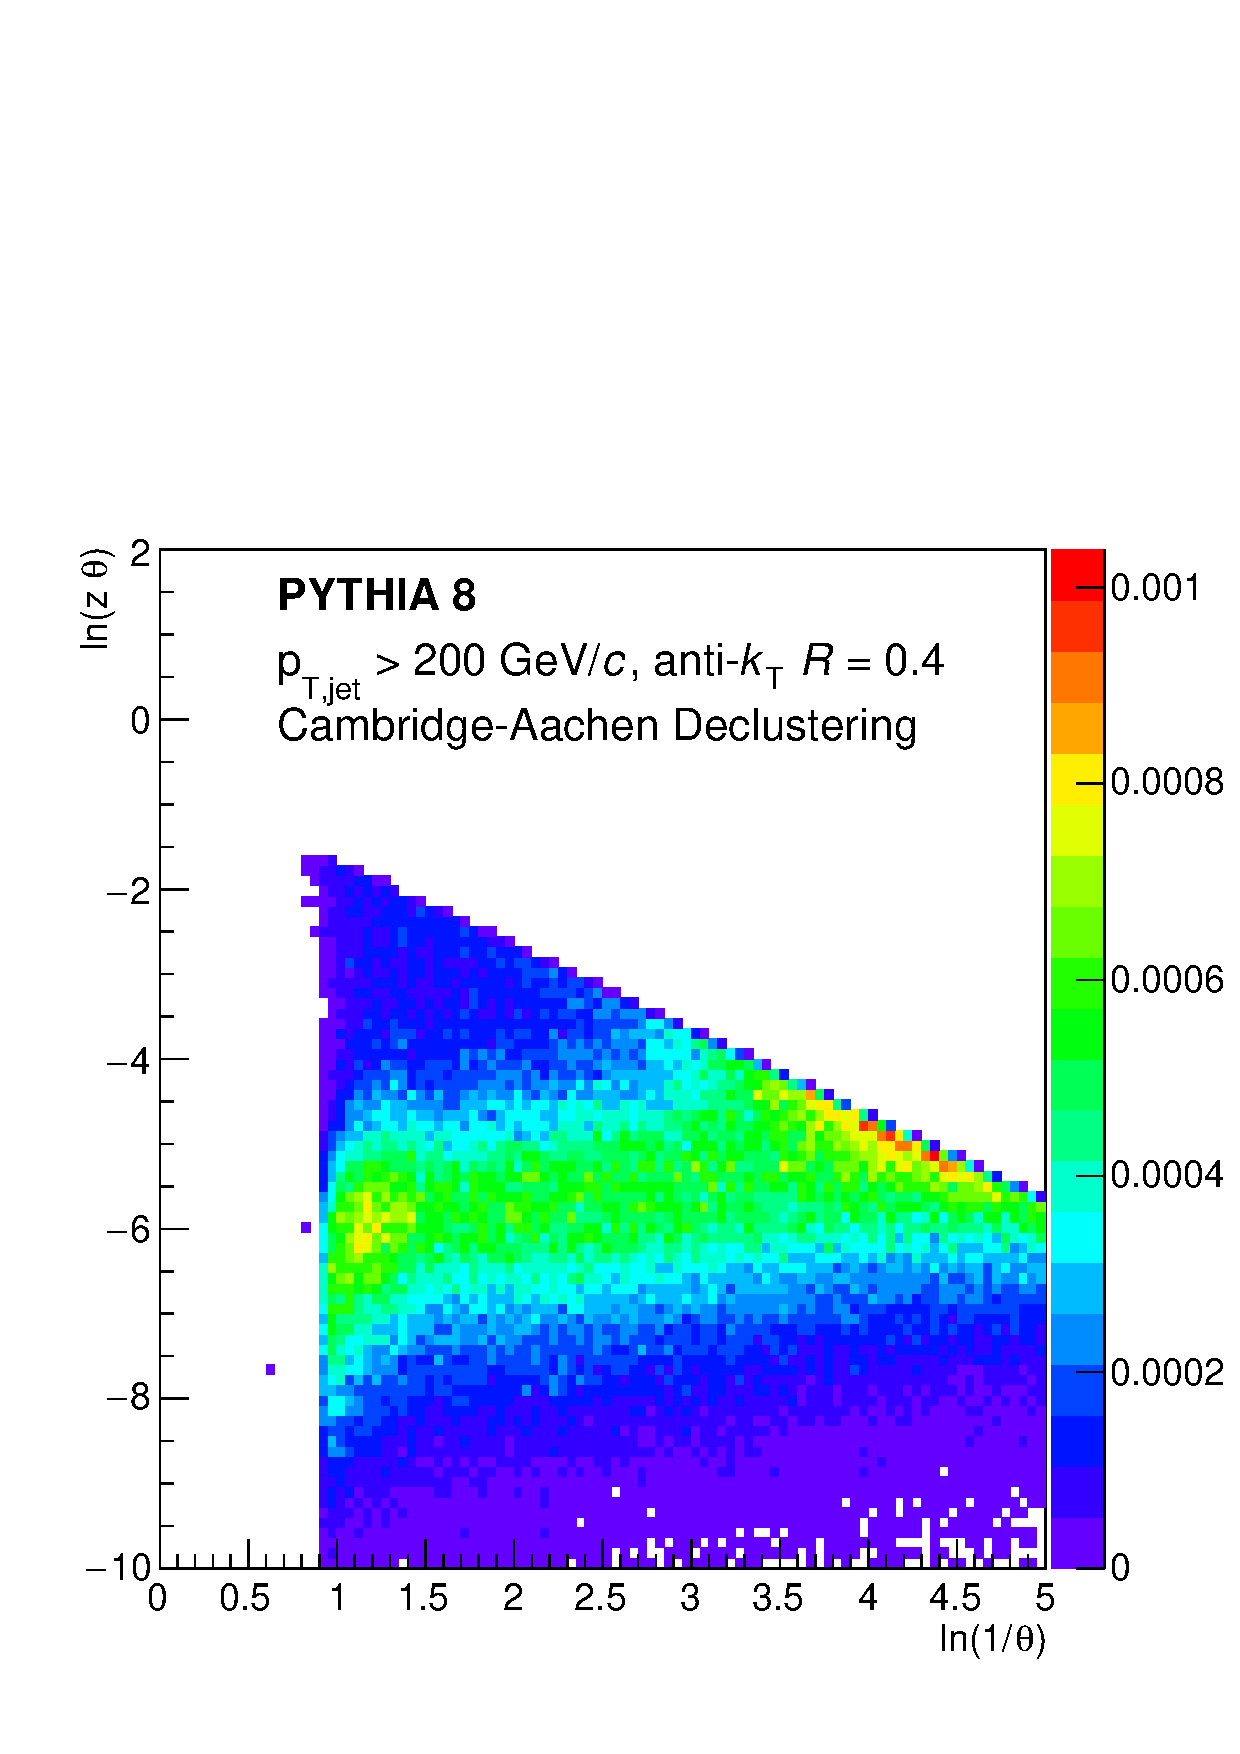
\includegraphics[width=0.4\textwidth]{figures/LundMC/Pythia_NoUE}
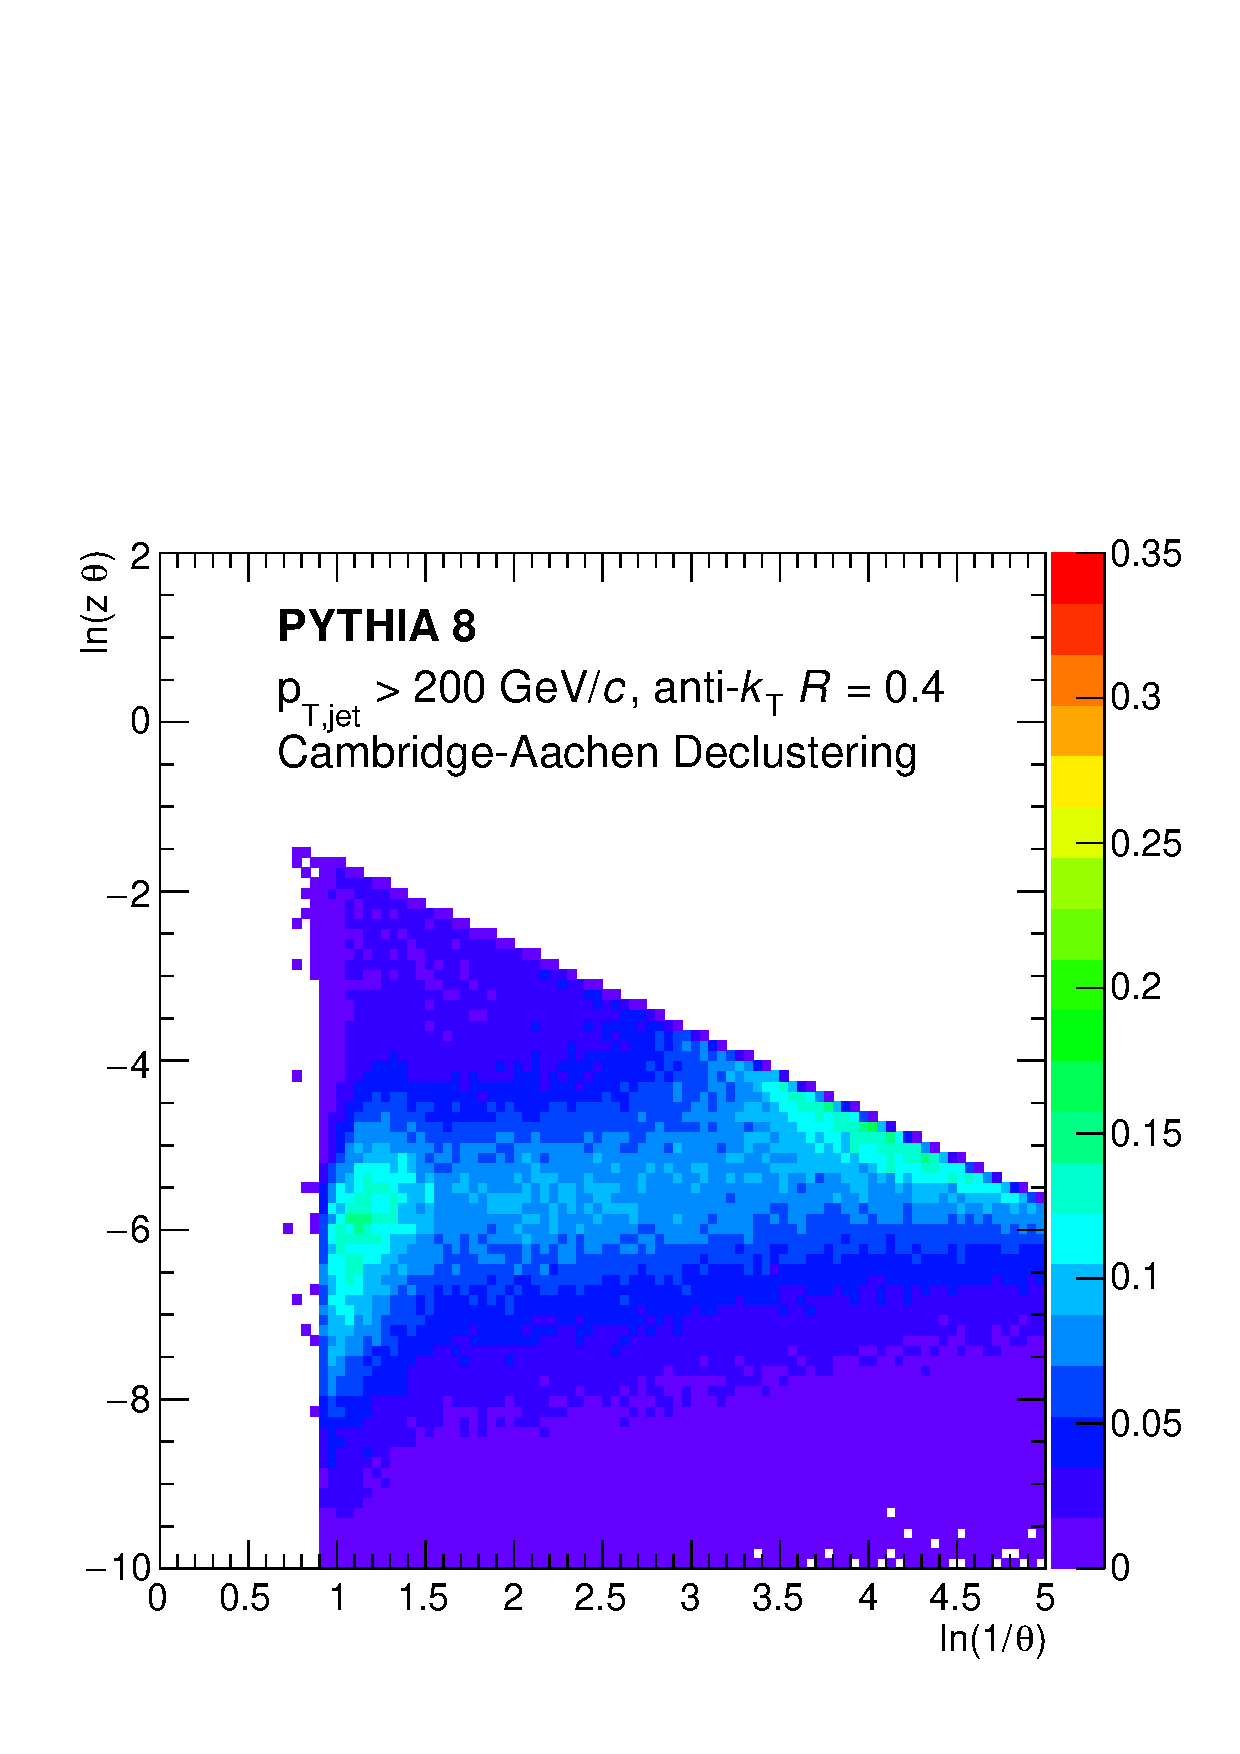
\includegraphics[width=0.33\textwidth]{figures/LundMC/FinalPlots/Pythia_CA.pdf}%
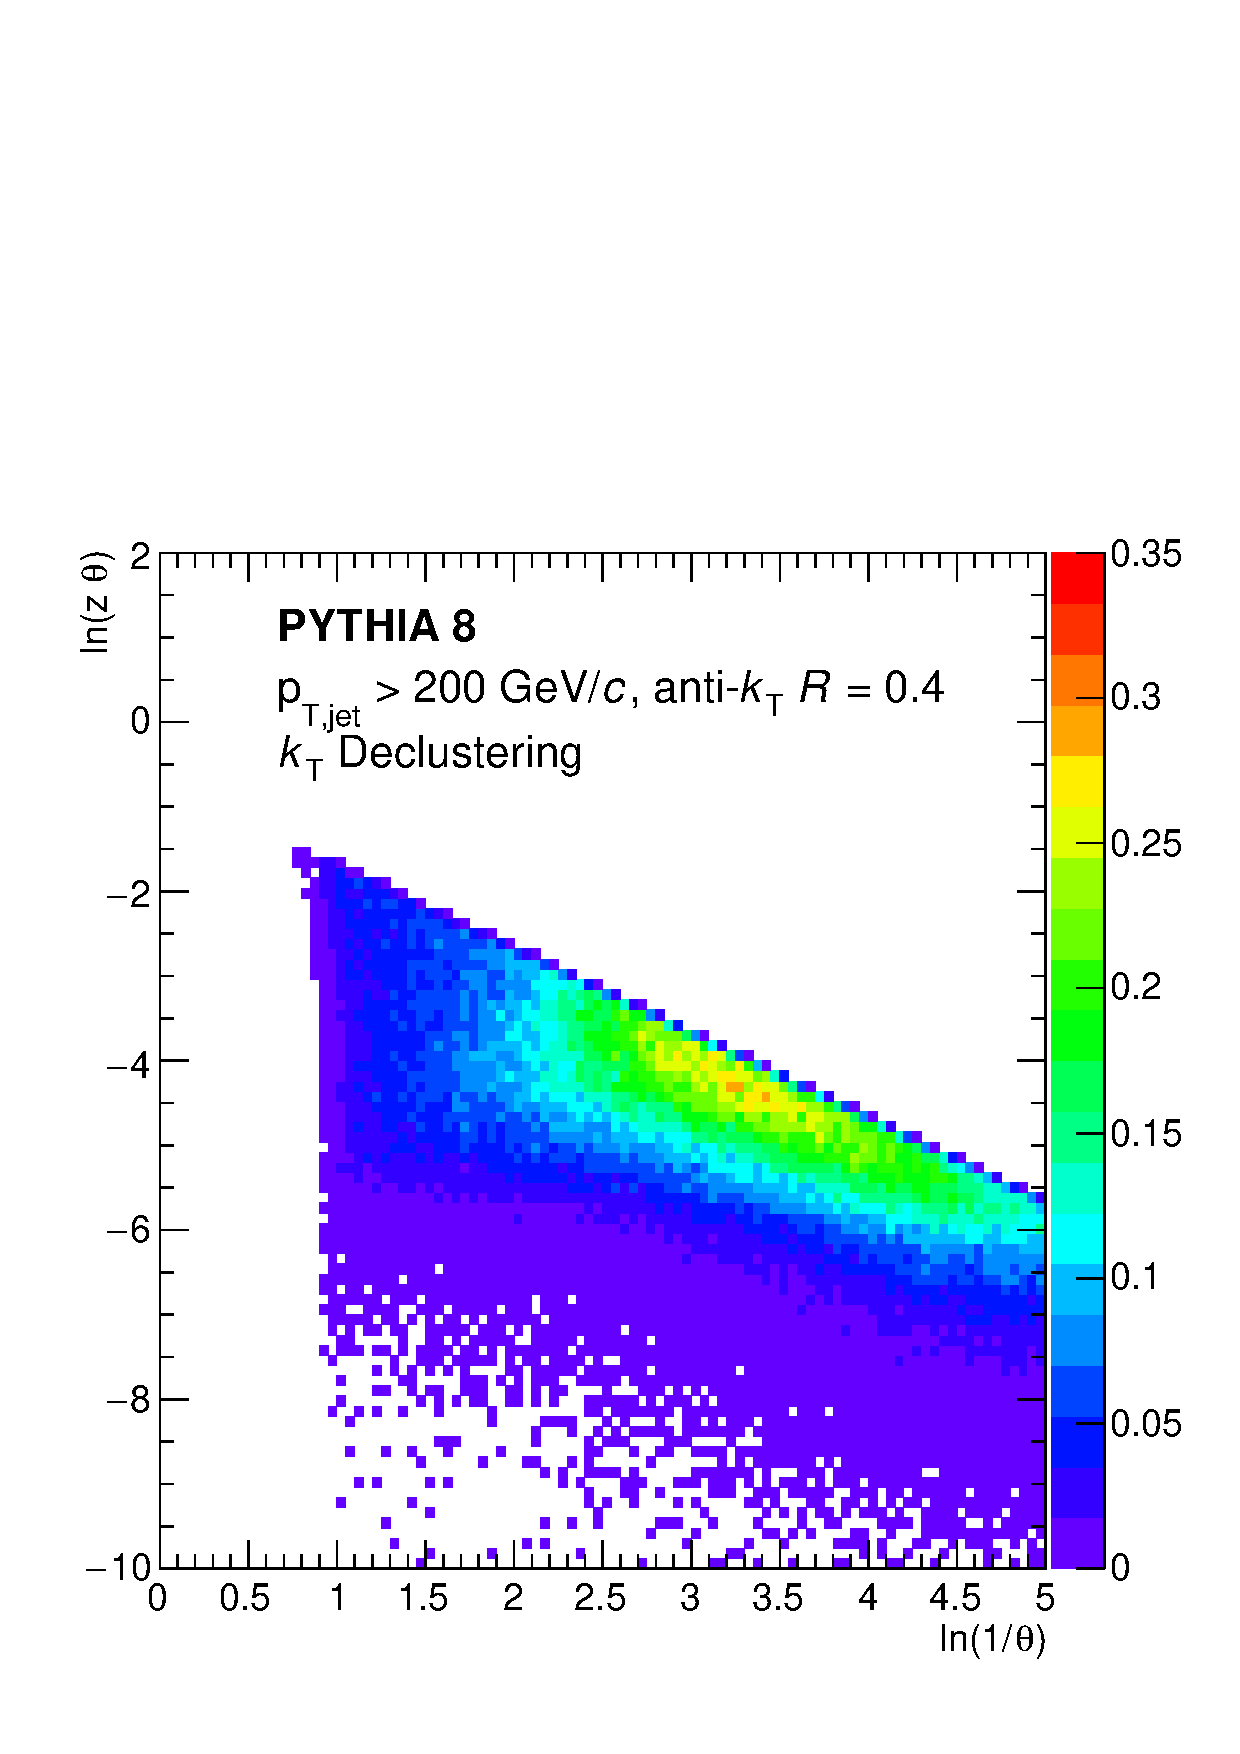
\includegraphics[width=0.33\textwidth]{figures/LundMC/FinalPlots/Pythia_kt.pdf}%
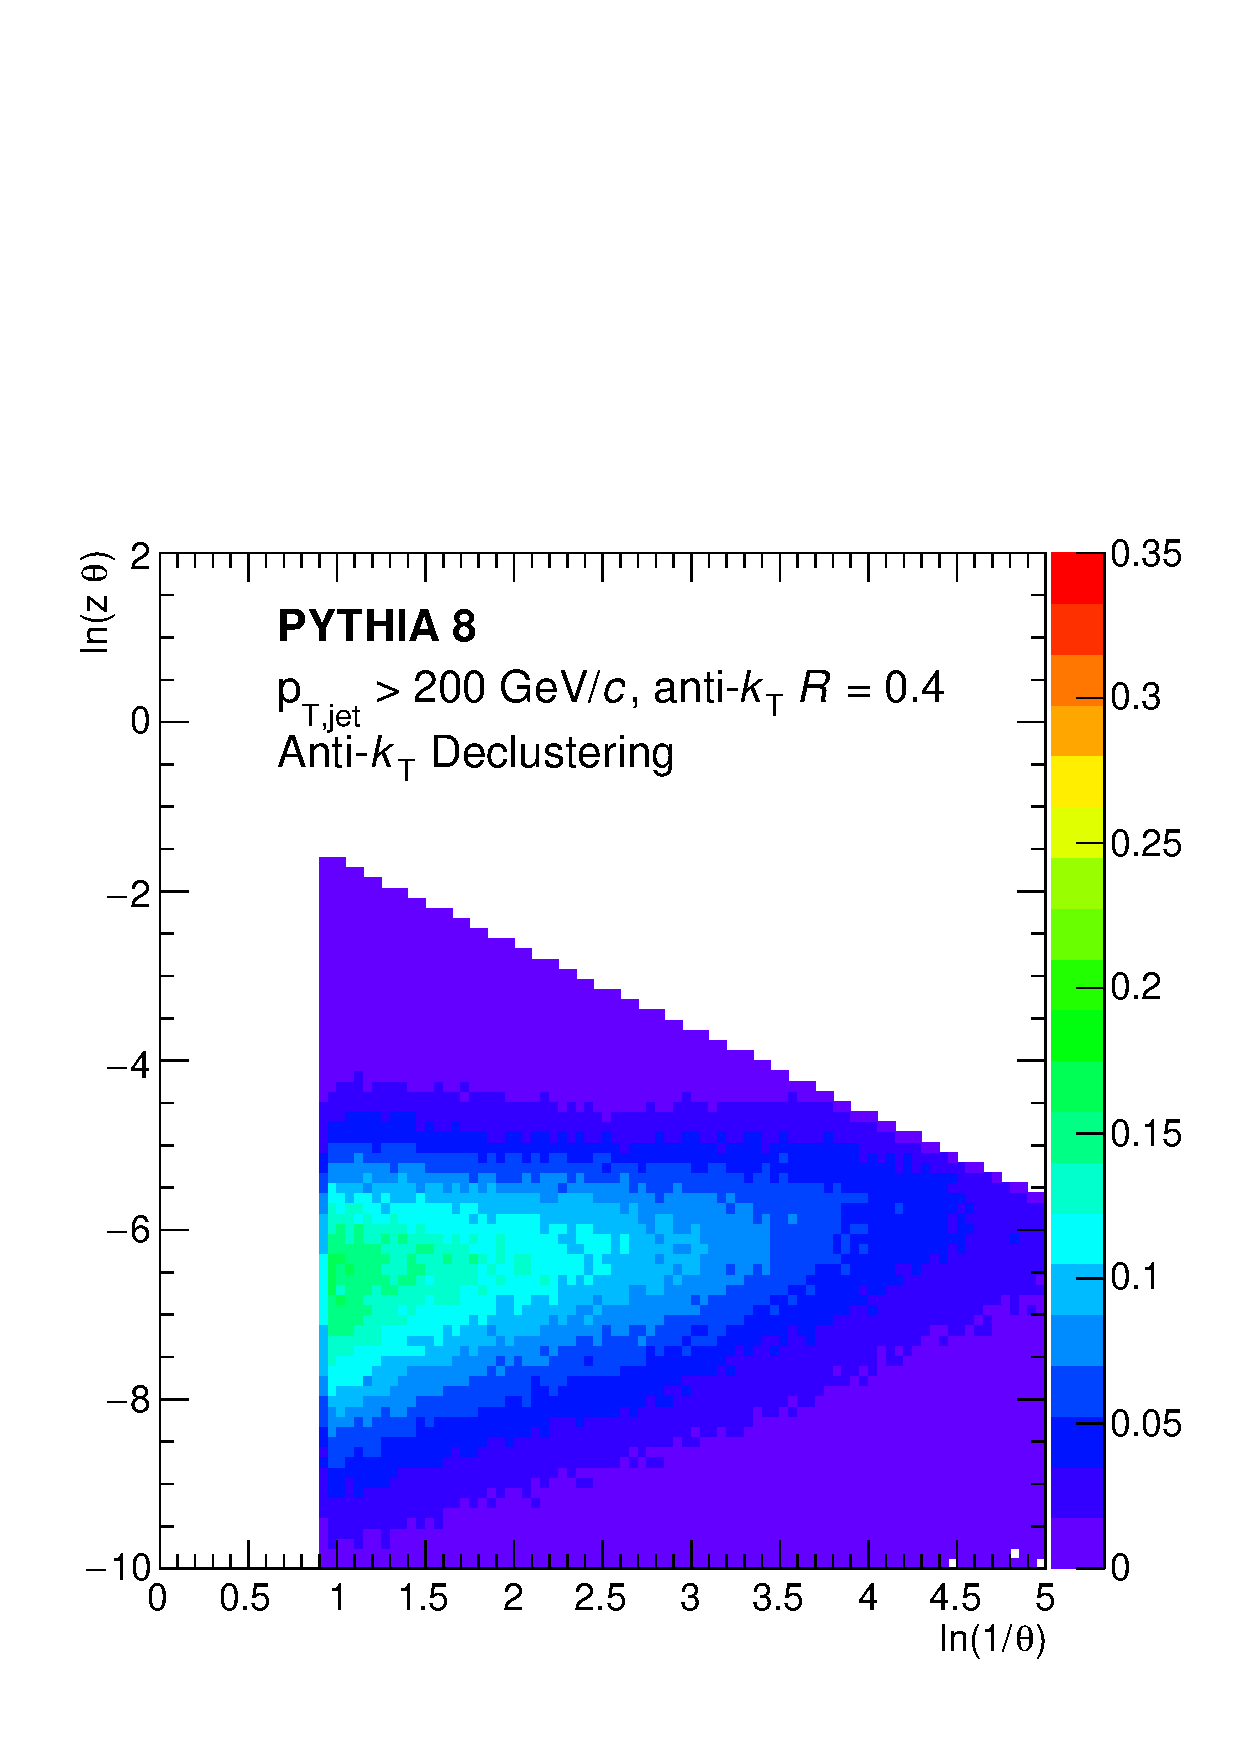
\includegraphics[width=0.33\textwidth]{figures/LundMC/FinalPlots/Pythia_Akt.pdf}%
\caption{Lund diagrams reconstructed from a sample anti-$k_{\rm \tiny T} = 0.4$ jets generated by PYTHIA8. Three reclustering strategies were considered: C/A (left), $k_{\rm \tiny T}$(middle), and anti-$k_{\rm \tiny T}$ (right).}
\label{fig:PS2Vac}
\end{figure}
%%%%%%%%%%%%%%%%%%%%%%%%%%%%%%%%%%%%%
Using this procedure for the three different reclustering algorithms, we analyzed a sample of jet generated by PYTHIA in \autoref{fig:PS2Vac}. The jet sample corresponds to reconstructed anti-$k_{\rm \tiny T} = 0.4$ jets with $\pT > 200 $ GeV/c. The expected, simple features are nicely realized for the C/A reclustering, see \autoref{fig:PS2Vac} (left). In particular, we see a slow enhancement of radiation at fixed $\kT$ which can mainly be attributed to running-coupling effects. The additional features can be attributed to effects from the underlying event that was not subtracted in this sample. Indeed, the maps generated by the (anti-)$k_{\rm \tiny T}$ reclustering are not uniform and possess and enhanced sensitivity to collinear, \autoref{fig:PS2Vac} (center), and soft, large-angle configurations, \autoref{fig:PS2Vac} (right), as naively expected.
See also \autoref{sec:reclusteringalgo}

As pointed out before, medium-induced radiation does not per se follow the same (angular) ordering as described above. In fact, the resummation of soft radiation leads to quite different characteristics. We will however continue to apply the procedure outlined above to identify regions of particular medium modification in the following Section. 
%Varying the reclustering algorithm can potentially enhance the sensitivity to different regimes, as found in the study above.


%{\color{red} Connect to discussion in the following sections.}

%%%%%%%%%%%%%%%%%%%%%%%%%%%%%%%%%%%%%%%%%
\subsection{Radiation phase space and sensitivity to jet quenching}
\label{sec:phasespace-mc}
%%%%%%%%%%%%%%%%%%%%%%%%%%%%%%%%%%%%%%%%%


%%%%%%%%%%%%%%%%%%%%%%%%%%%%%%%%%%%%%
\begin{figure}[h]
\centering
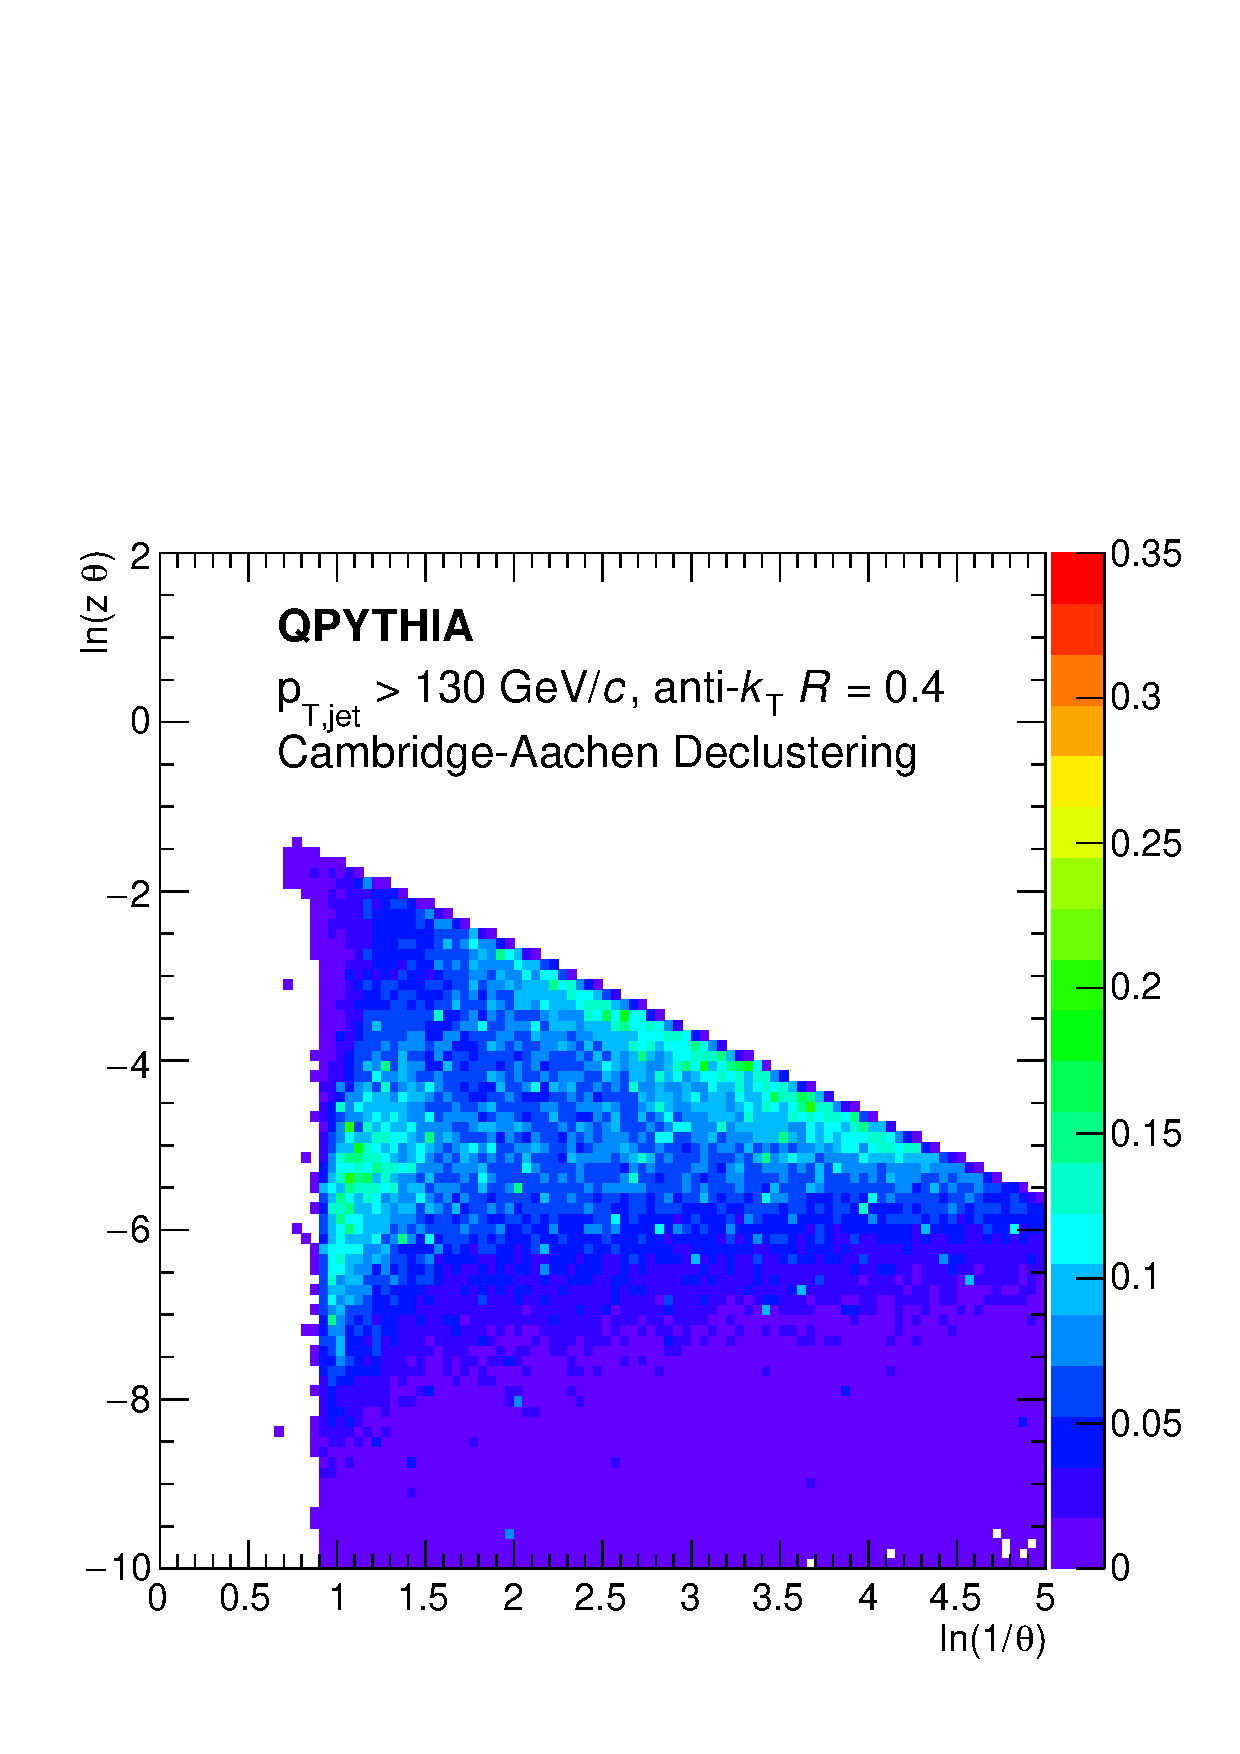
\includegraphics[width=0.3\textwidth]{figures/LundMC/FinalPlots/QPythia_Med.pdf}
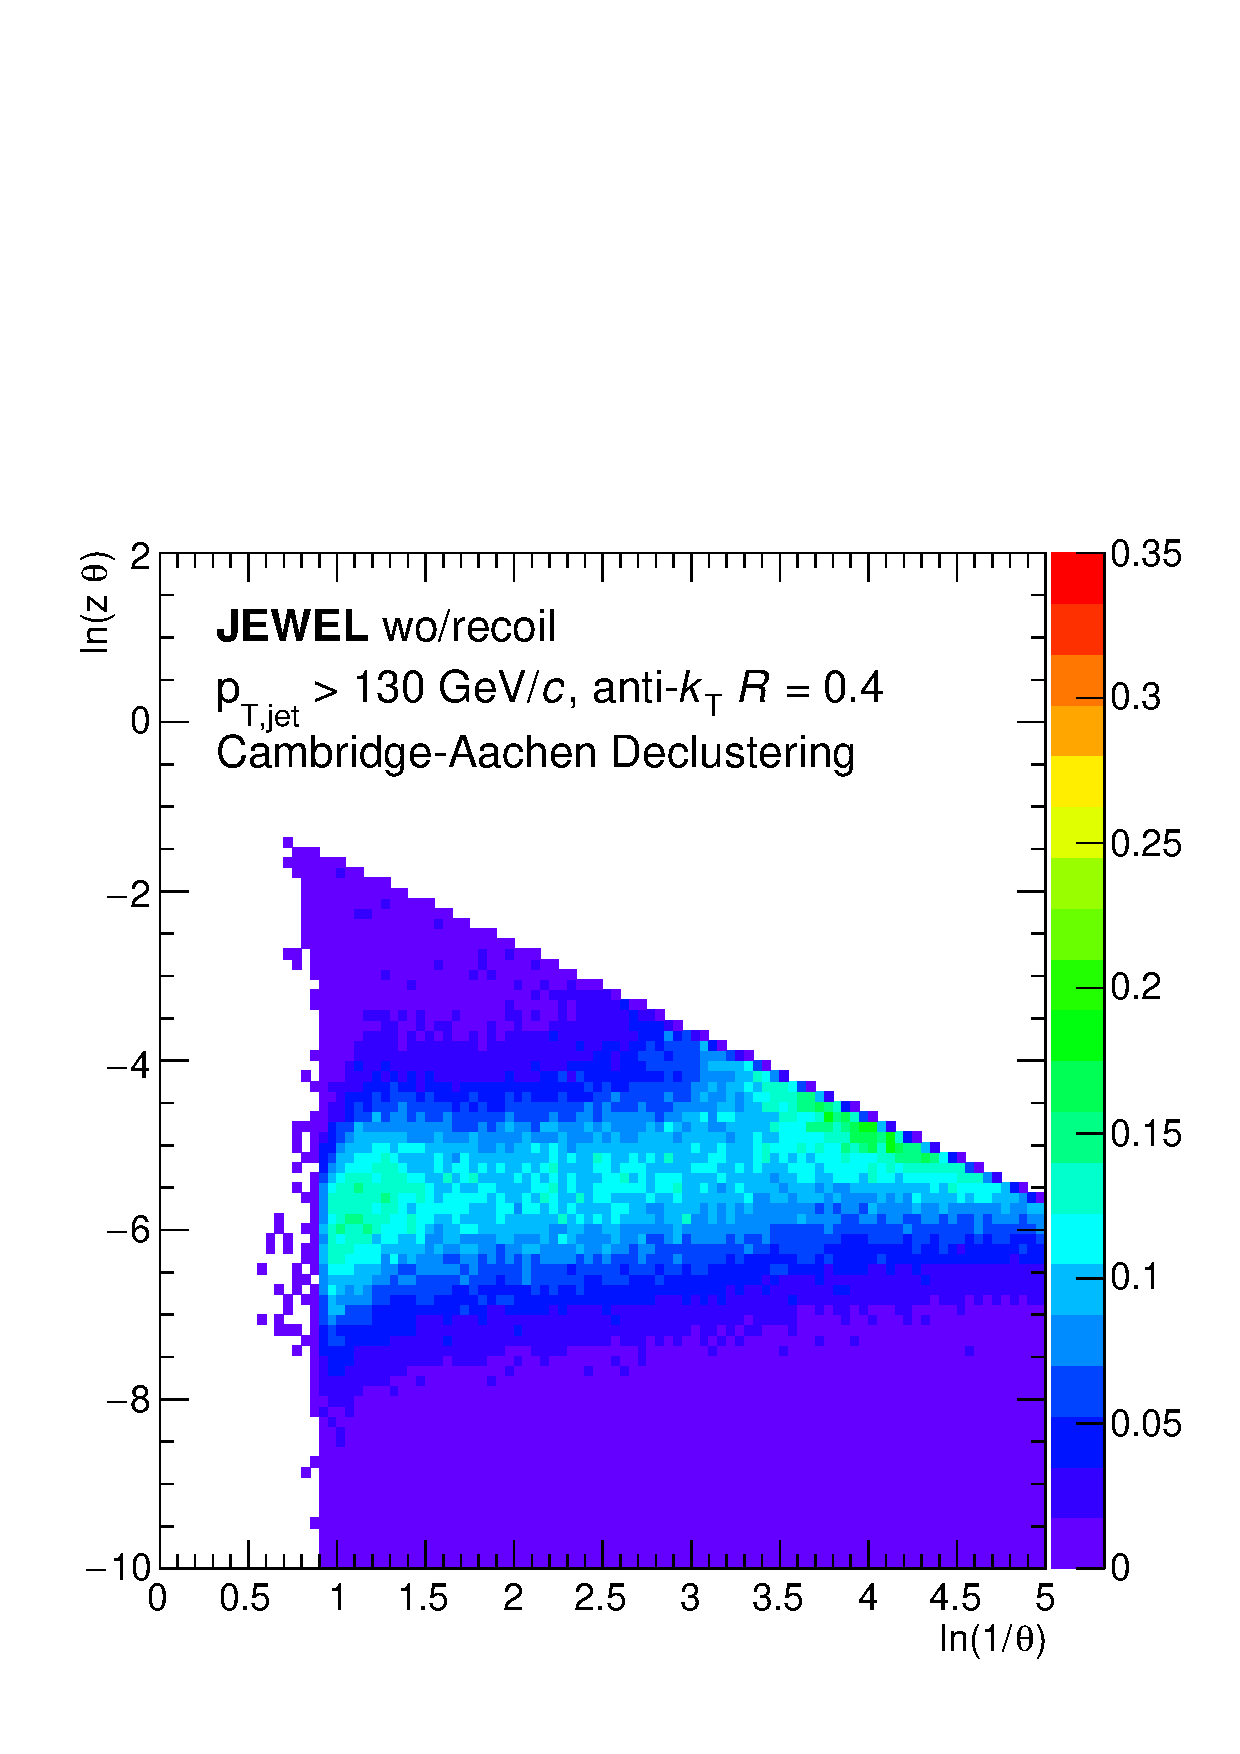
\includegraphics[width=0.3\textwidth]{figures/LundMC/FinalPlots/Jewel_Med_RecoilOff.pdf}
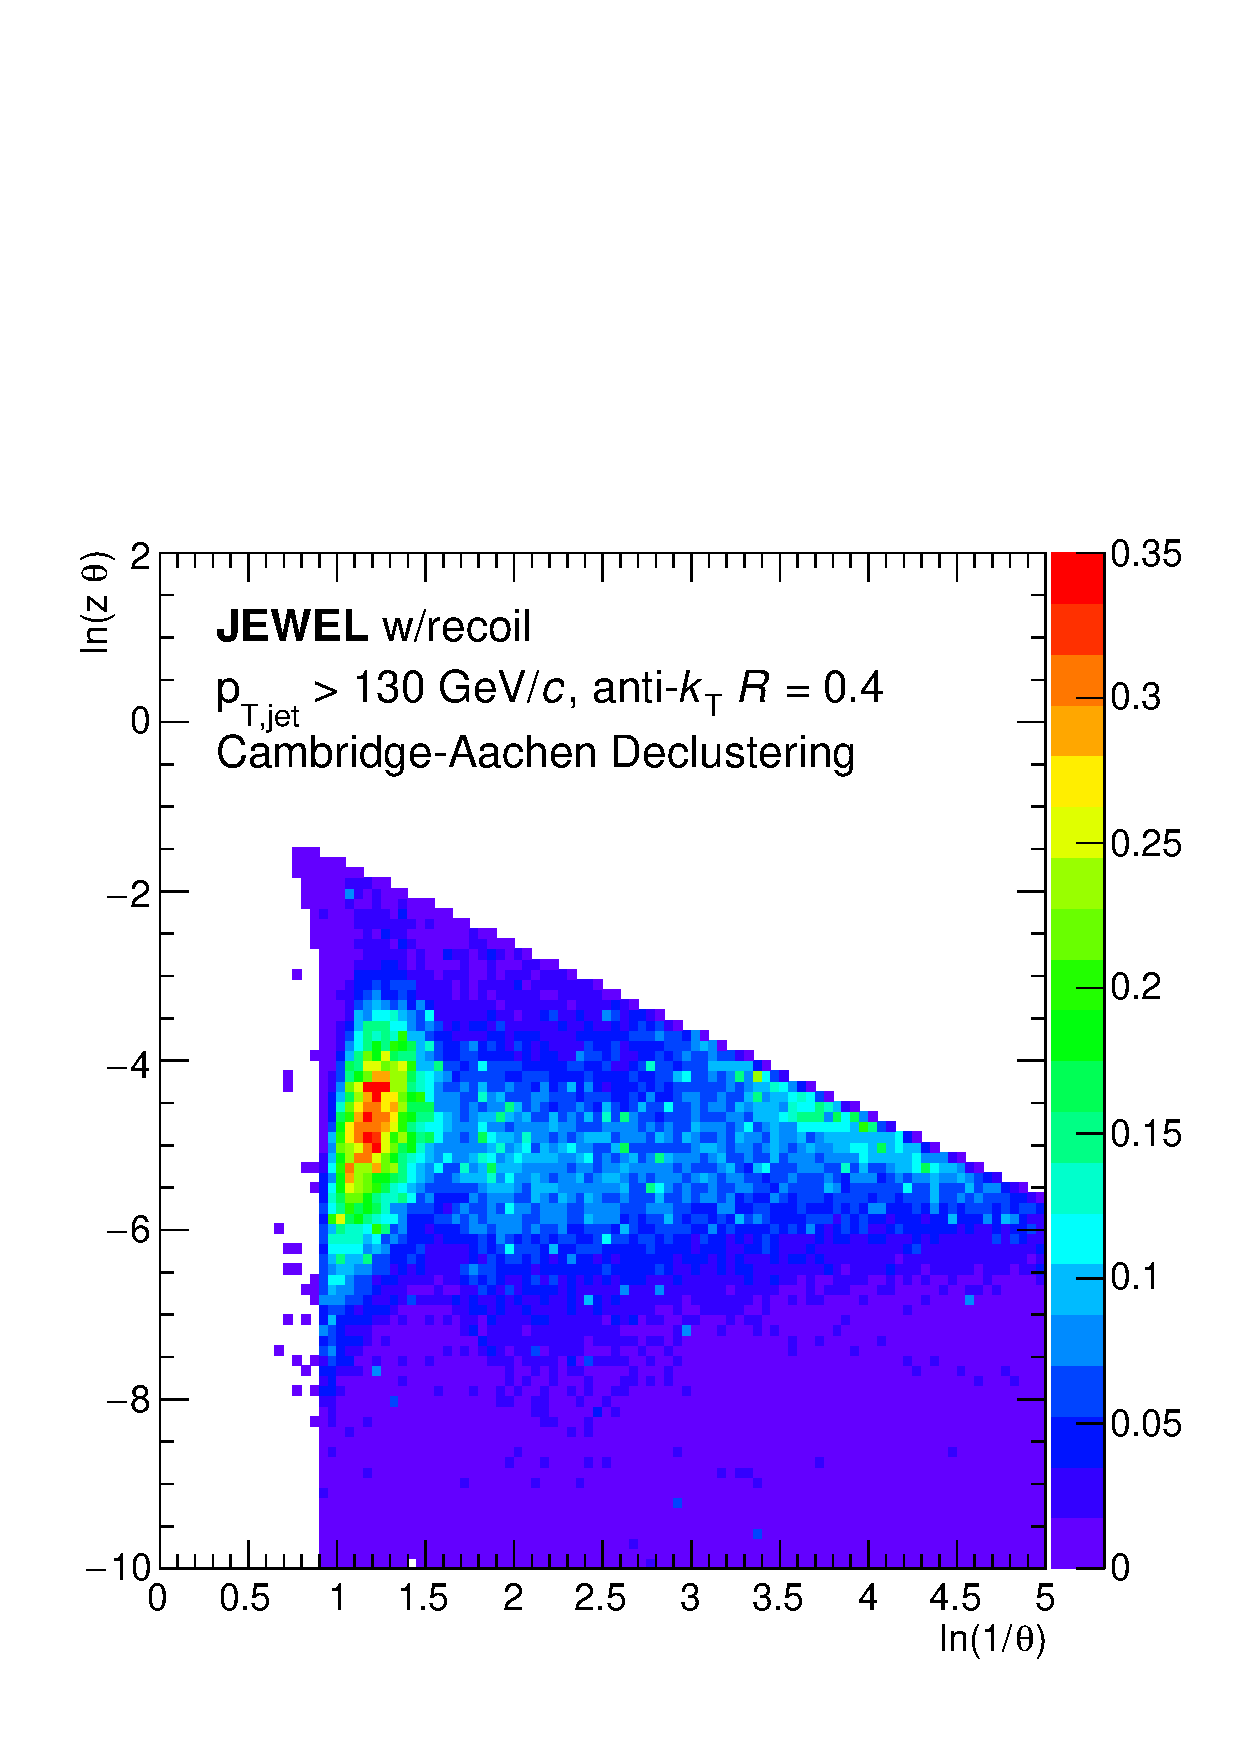
\includegraphics[width=0.3\textwidth]{figures/LundMC/FinalPlots/Jewel_Med_RecoilOn.pdf}
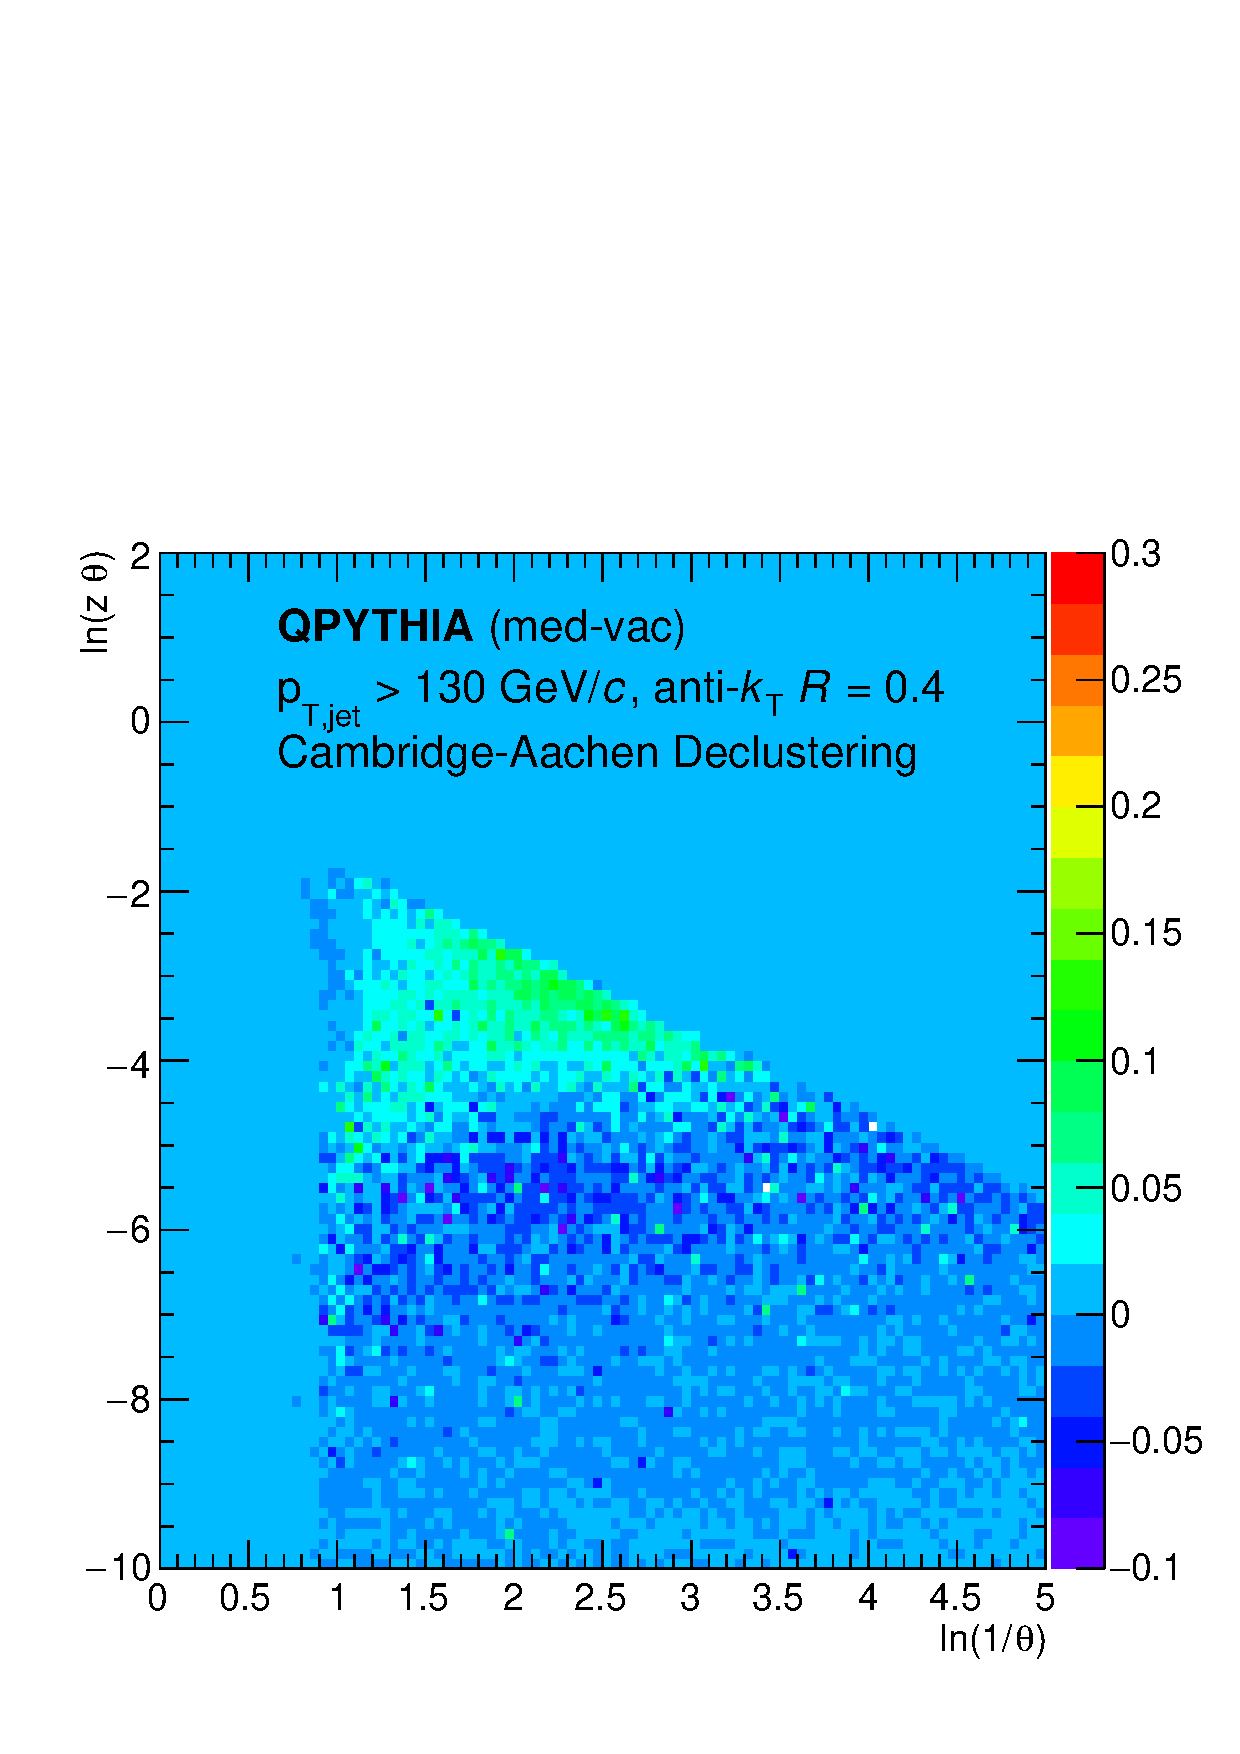
\includegraphics[width=0.3\textwidth]{figures/LundMC/FinalPlots/QPythia_Diff.pdf}
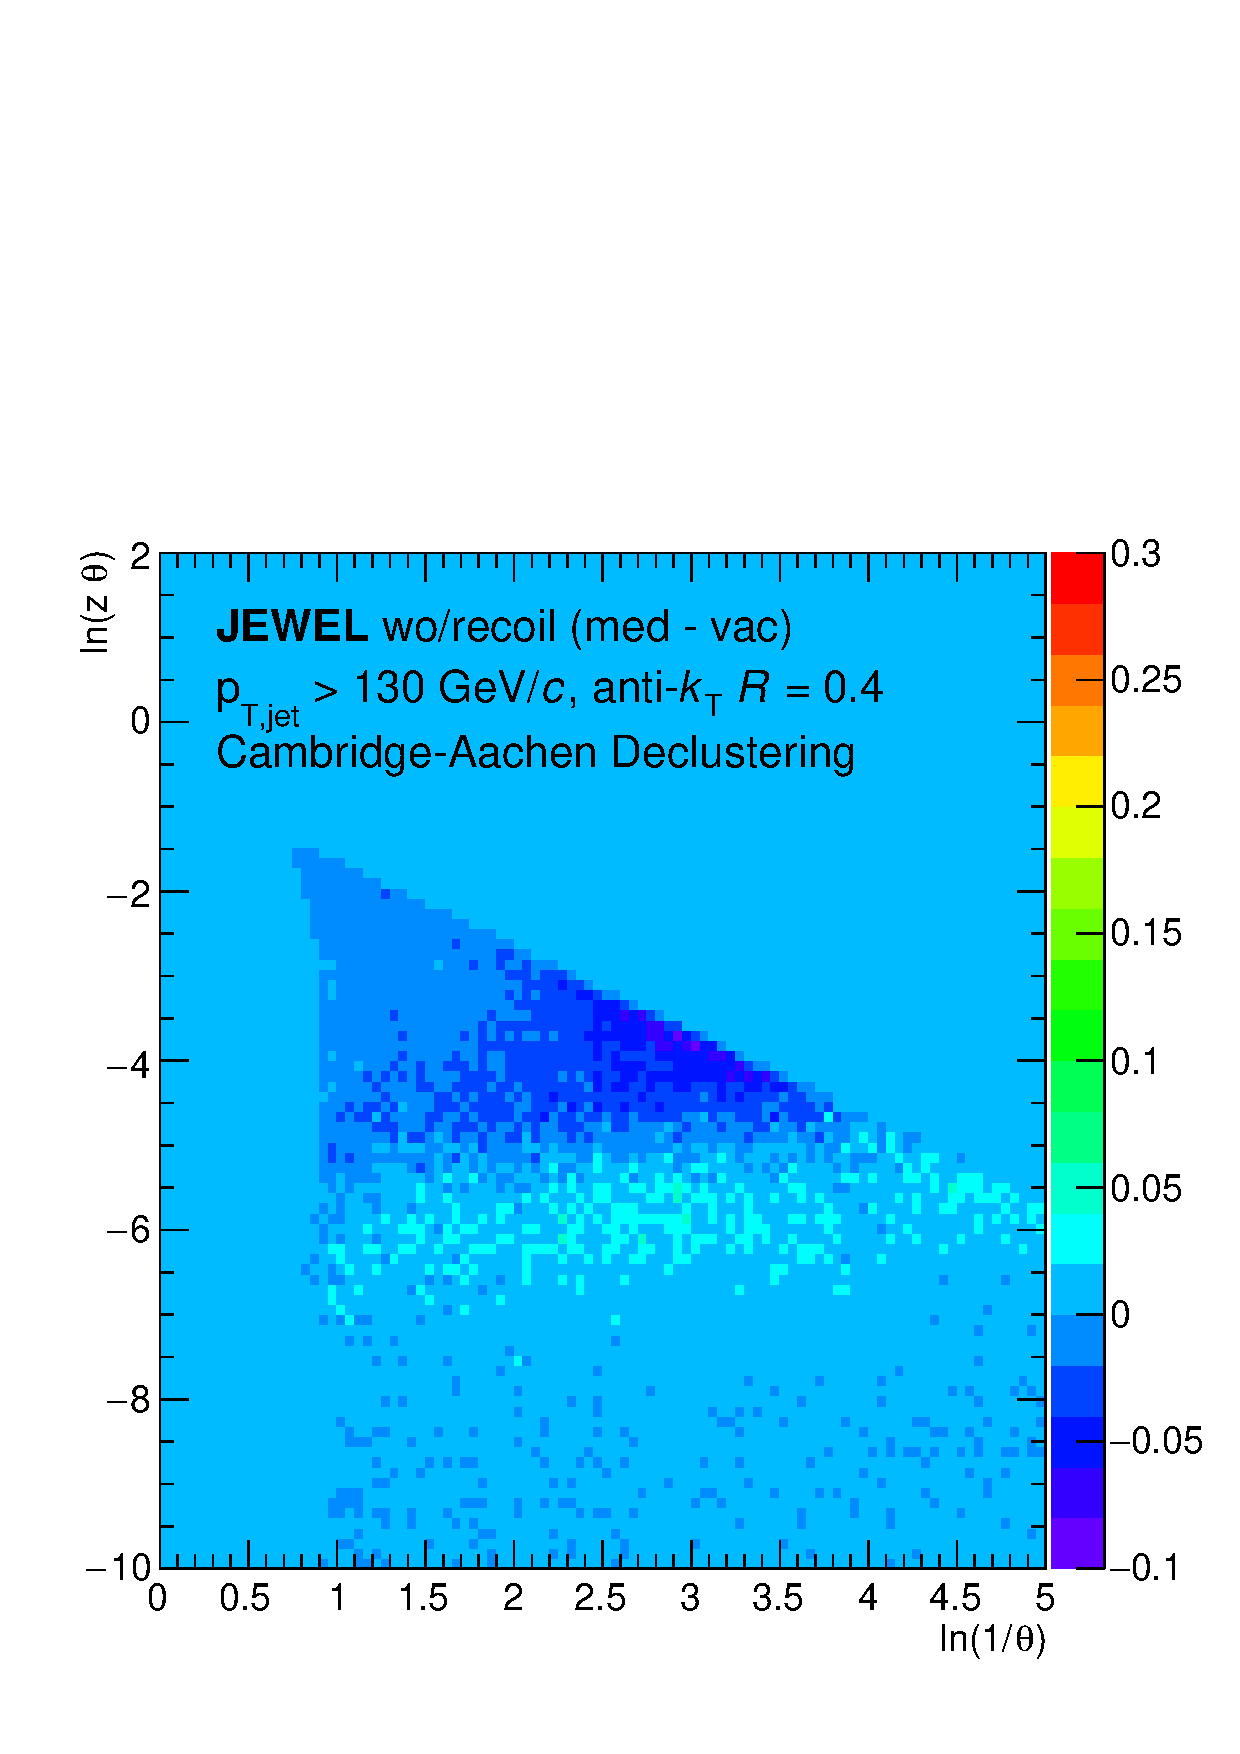
\includegraphics[width=0.3\textwidth]{figures/LundMC/FinalPlots/Jewel_Diff_RecoilOff.pdf}
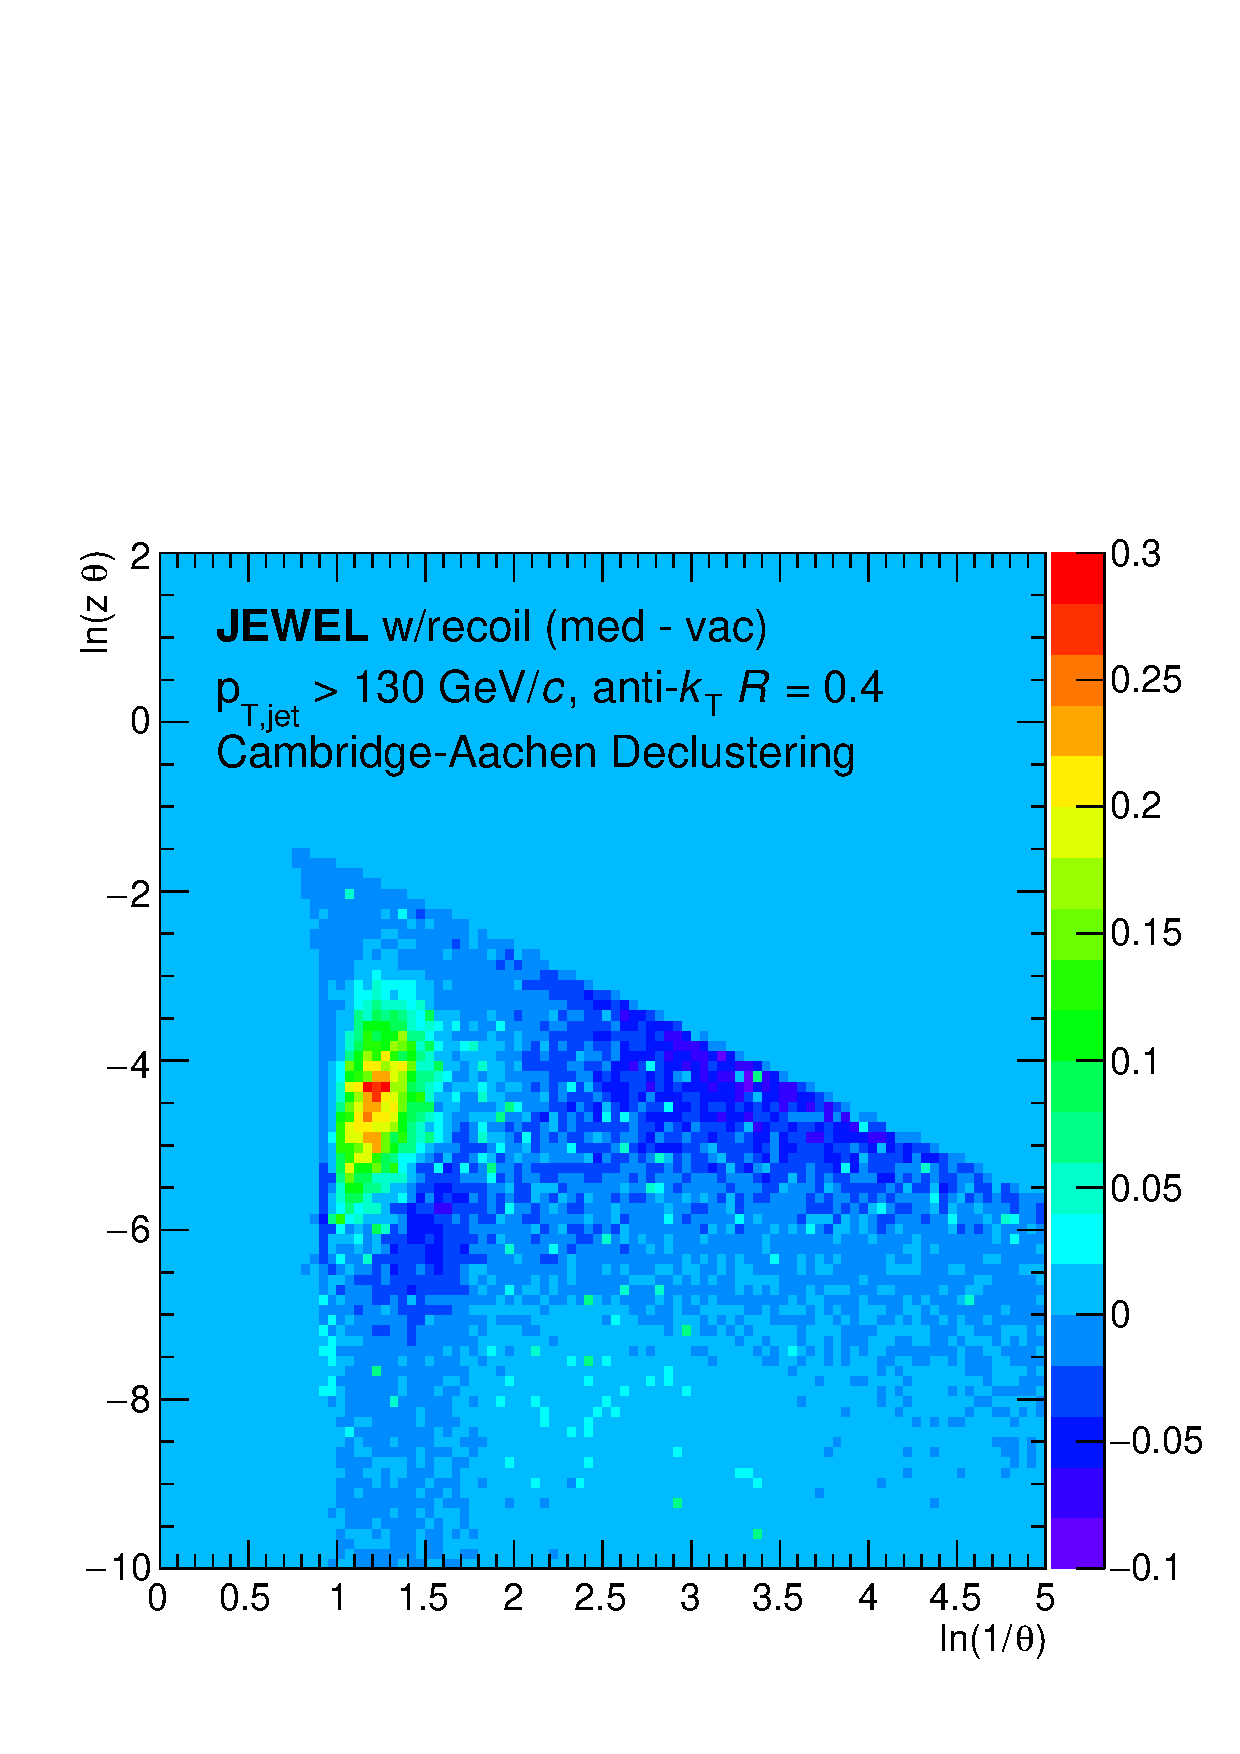
\includegraphics[width=0.3\textwidth]{figures/LundMC/FinalPlots/Jewel_Diff_RecoilOn.pdf}
\caption{Lund diagram reconstructed from jets generated by QPYTHIA (left column), JEWEL without recoils (middle column) and JEWEL with recoils (right column).
The lower panels correspond to the difference of the radiation pattern with and without jet quenching effects. Note that the scale of the $z$-axes varies between the panels.}
\label{fig:PS2}
\end{figure}
%%%%%%%%%%%%%%%%%%%%%%%%%%%%%%%%%%%%%
As a demonstration of the general ideas outlined above, we fill the Lund diagram using 
%PYTHIA 8, and 
two pQCD-based models for jet quenching, namely QPYTHIA \cite{Armesto:2009fj} and JEWEL \cite{Zapp:2011ya,Zapp:2012ak}. 
Both models implement the possibility for medium-induced bremsstrahlung. The latter model provides the possibility to track recoiling medium constituents that have interacted with the jet and, finally, include them in the hadronization step. 
%Jet quenching is expected to be accompanied by recoil effects. 
Hence, the jet-induced medium response constitutes a correlated background that can contribute to the modifications of the measured jet substructure. In the ``recoil off'' mode, the model only contains an additional radiative component with respect to vacuum.
Recoil effects are expected to contribute in the soft-large angle sector of the phase space, similarly to the uncorrelated underlying event, discussed further in \autoref{sec:uncorrelatedbackground}.
%in the next section. 
We refer to the two possibilities as ``Recoil on'' and ``Recoil off''. For further details regarding the models, see \App{app:models}.
% The variables $z\theta$ and $\theta$ have been reconstructed from subsequent branchings that were identified by reclustering the jet with a C/A algorithm.

%Fig.~\ref{fig:PS2Vac} shows the Lund diagram in vacuum and its characteristic horizontal bands due to the evolution of the coupling constant with the momentum scale are apparent. The excess of splittings at large angle seen in the left plot is caused by the PYTHIA underlying event, which is switched off in the right plot. 

For the same jet criteria as in \autoref{fig:PS2Vac}, in \autoref{fig:PS2} (upper row) we plot the Lund diagrams generated by QPYTHIA, JEWEL without recoils and JEWEL with recoils, respectively. 
\kmt{It should be pointed out specifically, one time, what version of JEWEL we are using, and which reference that corresponds to so that we, and the reader, can cross check our results.}
In this particular study, we focus on the C/A reclustering. The lower plots show the differences to the corresponding vacuum diagrams. The results from QPYTHIA exhibit an modest excess $\sim 10\%$ of hard quanta relative to vacuum, see \autoref{fig:PS2} (lower, left). In the model, the number of splittings is increased relative to vacuum leading to a significant intra-jet momentum broadening. 
%\sout{JEWEL generates additional medium-induced branchings that are not present in the vacuum reference. These are also allowed to branch further in the medium. In the difference plot we can clearly identify an excess $\sim 20\%$ of large-angle, semi-hard quanta in JEWEL, see \autoref{fig:PS2} (lower, center). This excess shows up at larger $k_\perp$ and is further enhanced $\sim 30\%$ when medium recoils are included, see Fig.~\ref{fig:PS2} (lower, right). }
%{\color{green} 
In the case of JEWEL, the difference plot does not show an increase of splittings but rather a small suppression $\sim 6\%$ of hard quanta, see \autoref{fig:PS2} (lower, center). This suppression is consistent with a lack of intra-jet broadening and a more collimated fragmentation. 
This shows that the realistic modifications to the Lund diagram are highly non-trivial and calls for a better theoretical understanding, see \autoref{sec:phasespace-theory} for a discussion.
When the medium recoils are included, an excess of semi-hard and large angle quanta appears, see \autoref{fig:PS2} (lower, right). 
We note that in our declustering approach the angles are always measured relative to the hardest parent or subjet, in which case the angular distribution can be broader than the angular distribution measured relative to the jet axis that is used to compute jet profiles , see for instance \cite{KunnawalkamElayavalli:2017hxo}.
%}
{\color{red} What is the interpretation of the enhancement/suppression wrt vacuum seen in QPYTHIA/JEWEL? How can we understand this in light of the discussion in Sec.~2 and Fig. 3? How do long-distance effects (broadening, recoil(?)) show up in the plane and ``ruin'' the space-time interpretation? How is energy loss affecting the plot? What would be the next step - more systematic studies, grooming studies of models, gen-level studies etc.!}

%The nature and role of the recoils will be explained in the next subsection. 

It is worth pointing out that the medium-induced signal populates different regions of phase space in the two jet quenching models. 
While these features ultimately will be reflected in the relevant observables, the mapping onto the Lund kinematical plane seem to be a powerful tool to identify the impact of various medium modifications. Performing additional grooming, that is picking out branchings with specific properties, allows to enhance the sensitivity to the signal depending on the grooming parameters, see \autoref{sec:jetsubstructure}. Furthermore, changing the reclustering algorithm could also boost the signal, cf. \autoref{fig:PS2Vac}.
%In Fig. \ref{fig:AlgoDependenceSignal}, left plot, the difference between JEWEL (recoils off) and vacuum is shown for k$_{T}$ declustering strategy. The similar plot for QPYTHIA is shown on the right plot. 
%\sout{We have seen that, in the case of JEWEL, the excess of large-angle splittings is of the same order of magnitude with C/A and $k_{\rm \tiny T}$ strategies. In the case of QPYTHIA, the excess of hard splittings is enhanced to $\sim 20\%$ with $k_{\rm \tiny T}$ reclustering.}
%{\color{green} 
We have seen that, in the case of JEWEL, the suppression of hard splittings is enhanced to $\sim 14\%$ with $k_{\rm \tiny T}$ reclustering. In the case of QPYTHIA, the excess of hard splittings is enhanced to $\sim 20\%$ with $k_{\rm \tiny T}$ reclustering.

The impact of the recoils as modeled by JEWEL has been extensively documented \cite{KunnawalkamElayavalli:2017hxo,Milhano:2017nzm}. Its contribution is needed to describe most of the jet shapes measured so far at the LHC. In particular, if the medium response can smear the subleading subjet momentum above the given grooming cut, the subjet momentum balance or $z_{g}$ can become more asymmetric relative to vacuum.   As a correlated background, the medium response cannot be experimentally subtracted to isolate purely radiative modifications to the jet shower. However, a cross-correlation of jet substructure observables might help to suppress its influence \cite{Milhano:2017nzm}.

It is worth noting that, albeit in a complicated form, the splitting map contains of the information about a given medium shower. Certainly, such a procedure can be directly applied to experimental data, apart from the aspect of uncorrelated background that we outline in the next Section. Hence, in the remaining part of the report, the observables we choose to analyze will reflect particular features that already appear in the splitting map.


%%%%%%%%%%%%%%%%%%%%%%%%%%%%%%%%%%%%%%%%
\subsubsection{Sensitivity to uncorrelated background}
\label{sec:uncorrelatedbackground}
%%%%%%%%%%%%%%%%%%%%%%%%%%%%%%%%%%%%%%%%

%%%%%%%%%%%%%%%%%%%%%%%%%%%%%%%%%%%%%%%%
\begin{figure}[th]
\centering
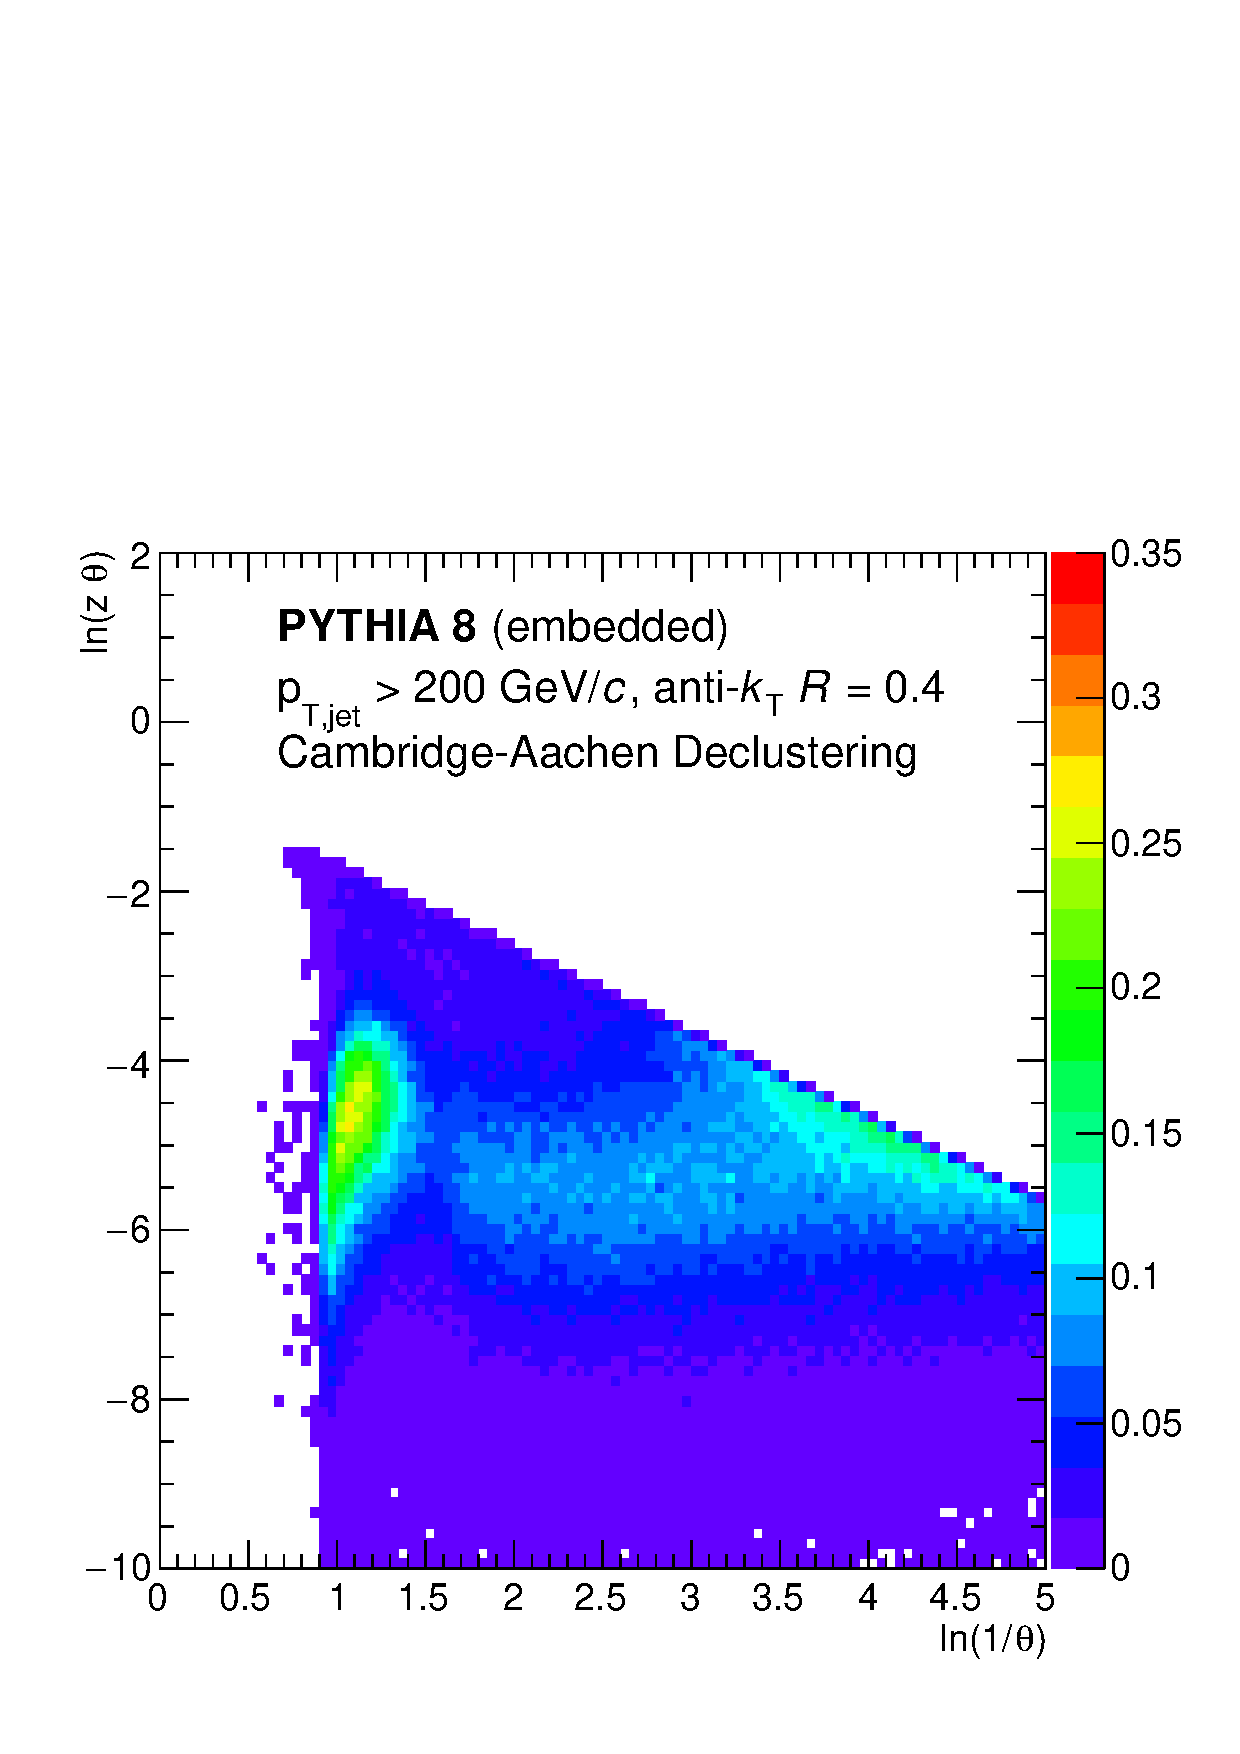
\includegraphics[width=0.33\textwidth]
{figures/LundMC/FinalPlots/PythiaEmb_CA.pdf}%
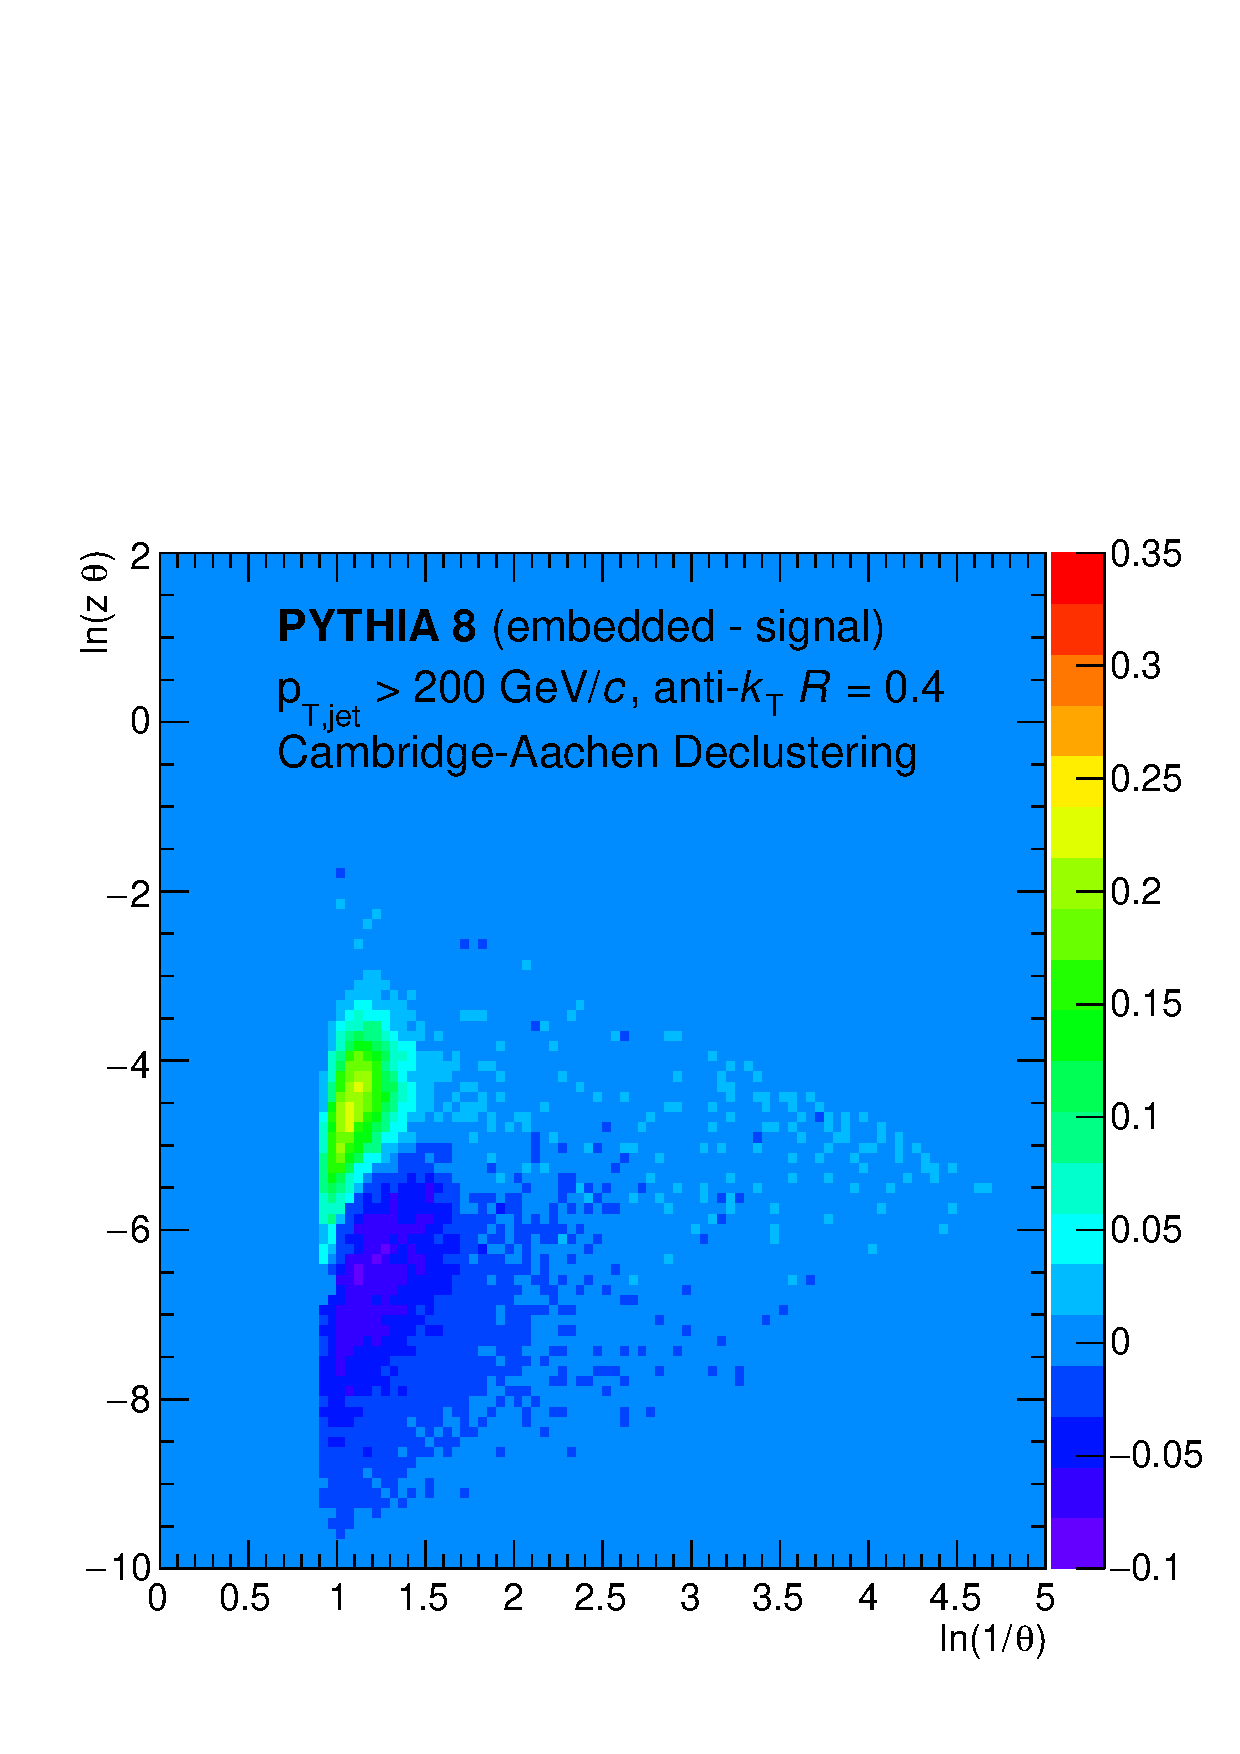
\includegraphics[width=0.33\textwidth]
{figures/LundMC/FinalPlots/PythiaDiff_CA.pdf}%
\caption{Impact of the uncorrelated background in the splitting map of the PYTHIA shower.}
\label{fig:UncorrelatedBkg}
\end{figure}
%%%%%%%%%%%%%%%%%%%%%%%%%%%%%%%%%%%%%%%%

In all the studies performed so far in this Section, we have not included the effect of considering a realistic heavy-ion background. In these studies, we have been using thermal events corresponding to a momentum density of $\rho =120$ GeV which corresponds to the most central events in the CMS detector, corresponding to a total multiplicity of $\sim 7000$ particles. 
{\color{red} More details on background, where do we take it from, parameters,  referecens etc.. Details on embedding...}

Hence, ending this section, we would also like to point out the fragility of using the Lund kinematical diagram in a realistic, noisy environment.
The heavy ion background that is uncorrelated to the jet will populate the phase space in the form of soft splittings at large angle $\theta \sim R$, where the area is maximal. Depending on the considered jet $p_{T}$, these fake splittings can contribute significantly to the distribution of groomed observables, cf. \autoref{sec:jetsubstructure}, by enhancing the number of asymmetric splittings and inducing a strong modification relative to vacuum jets. 
\autoref{fig:UncorrelatedBkg} shows the Lund diagram filled iteratively with PYTHIA jets embedded into a thermal background (left) and the difference plot to PYTHIA (right). The difference plot shows the enhancement of uncorrelated splittings at large angles. 
%Superimposed to the plot, the black line with negative slope sets the limits for the subsample of splittings that would be selected by grooming with default parameters and highlights the fraction of fake splittings that would enter the $z_{g}$ calculation. The plot on the right is filled with jets at lower energies and shows that the impact of the uncorrelated background increases as expected.
This provides a hint that, no matter the grooming settings, this becomes a significant contribution to the observable the smaller the $\pT$.

%%%%%%%%%%%%%%%%%%%%%%%%%%%%%%%%%%%%%%%%
\begin{figure}
\centering
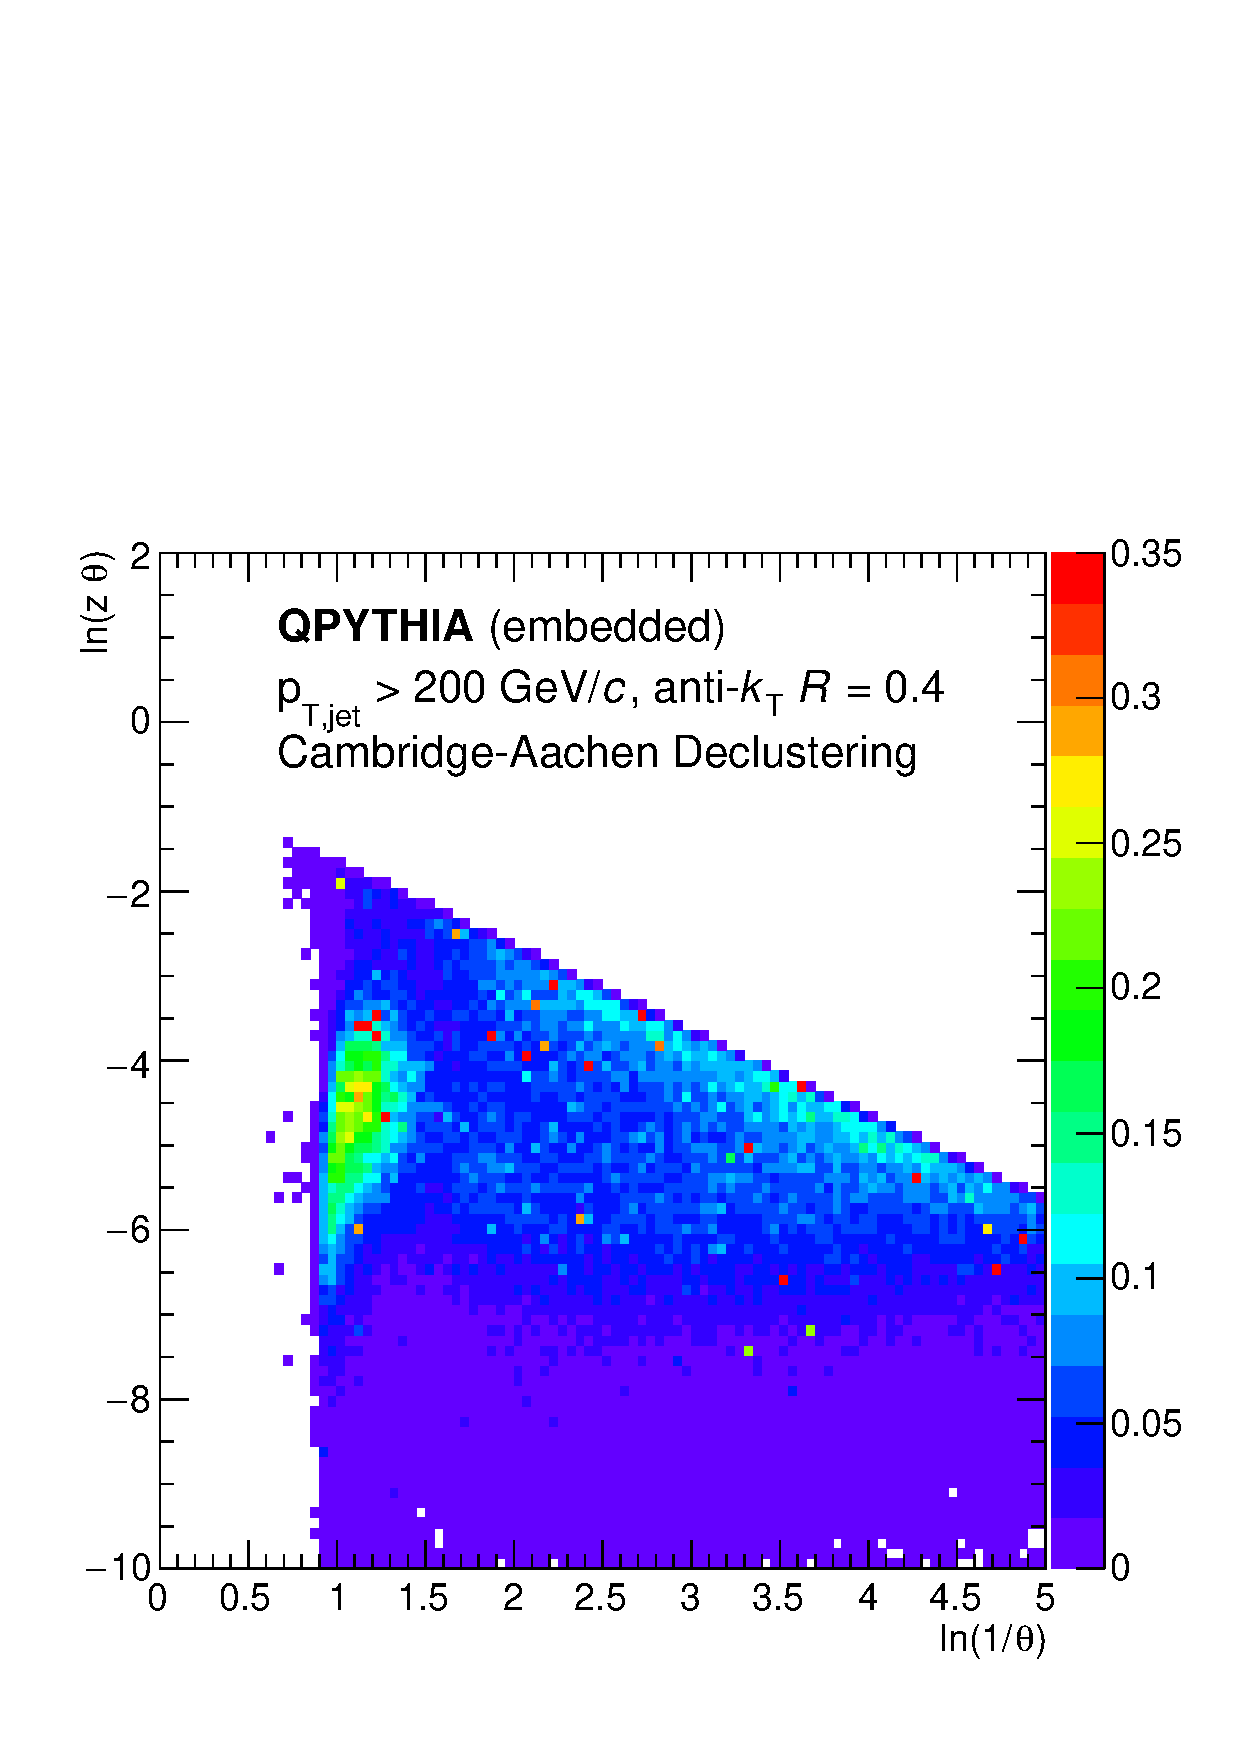
\includegraphics[width=0.32\textwidth]
{figures/LundMC/FinalPlots/QPythia_Emb.pdf}
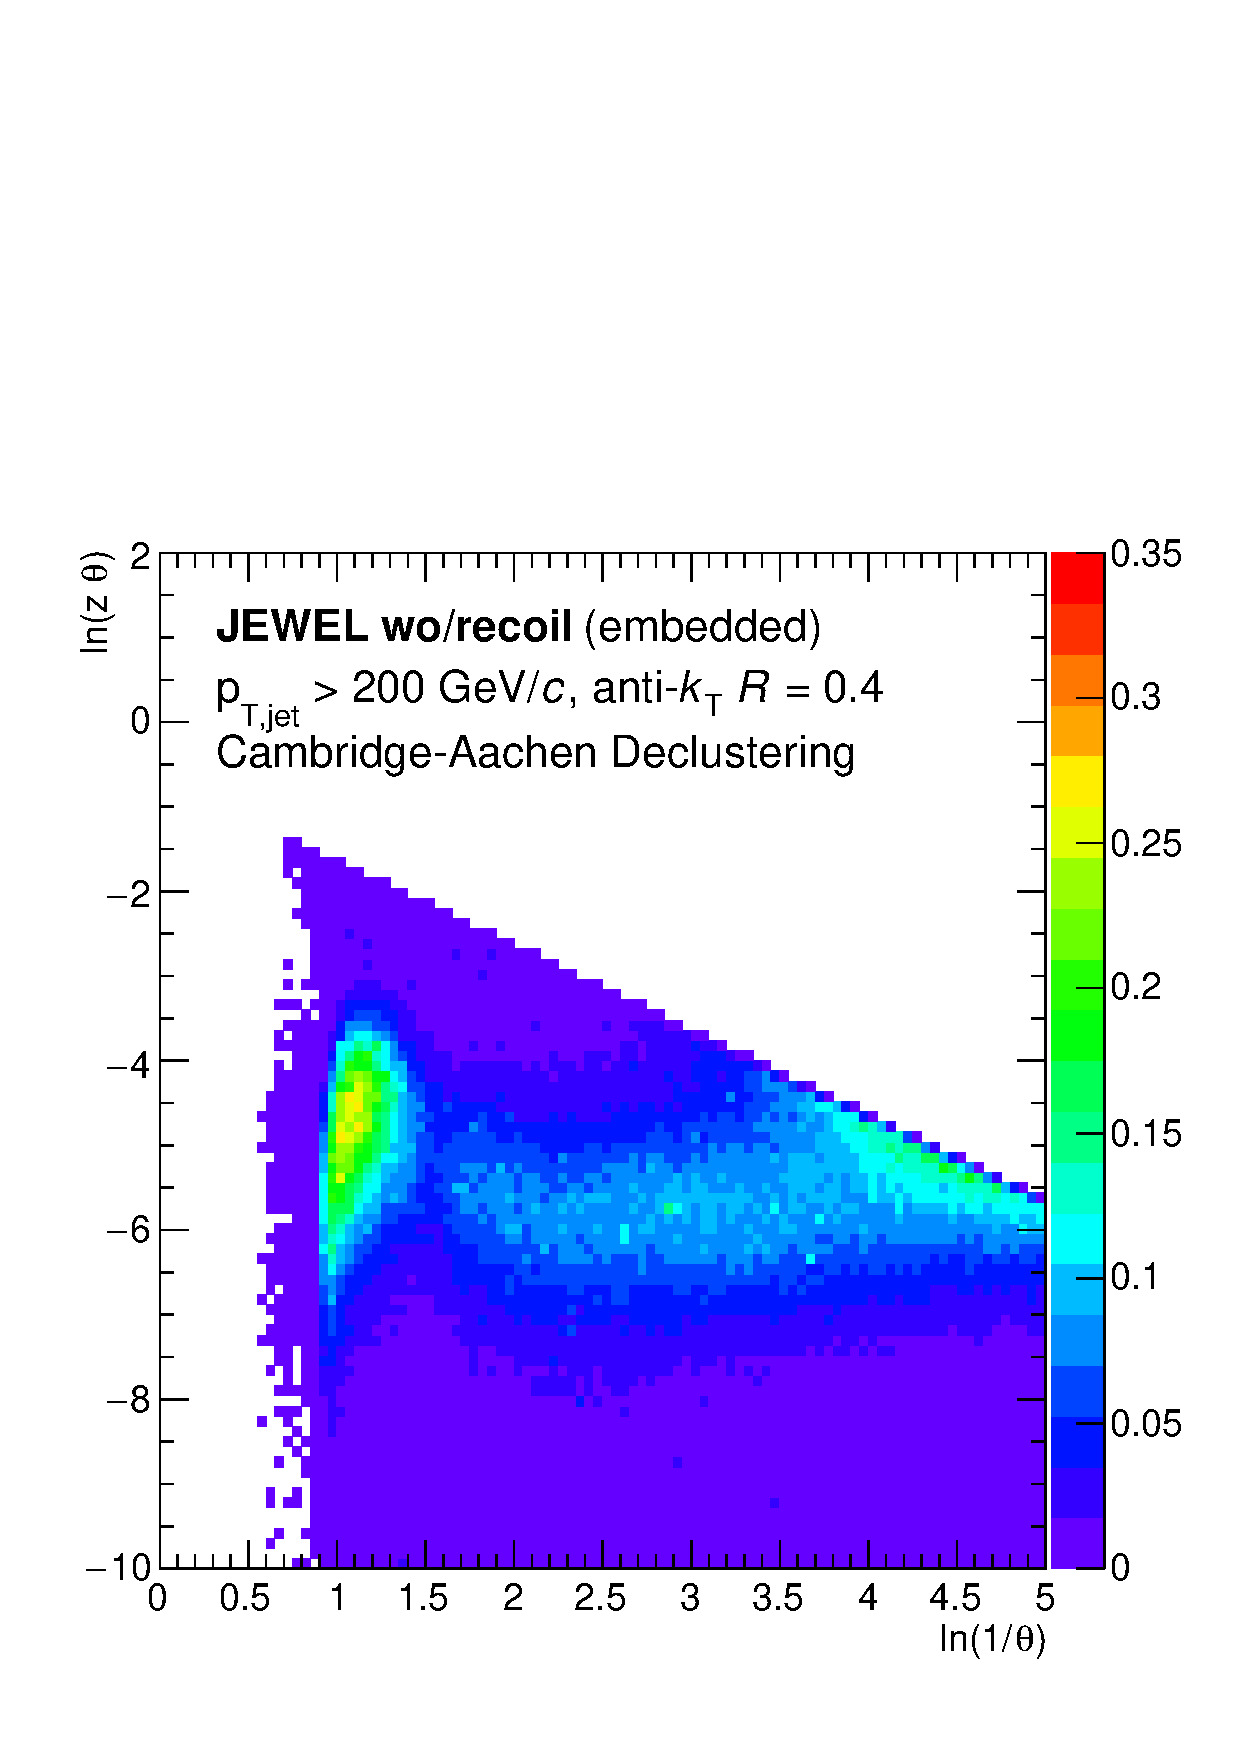
\includegraphics[width=0.32\textwidth]
{figures/LundMC/FinalPlots/Jewel_MedEmb_RecoilOff.pdf}
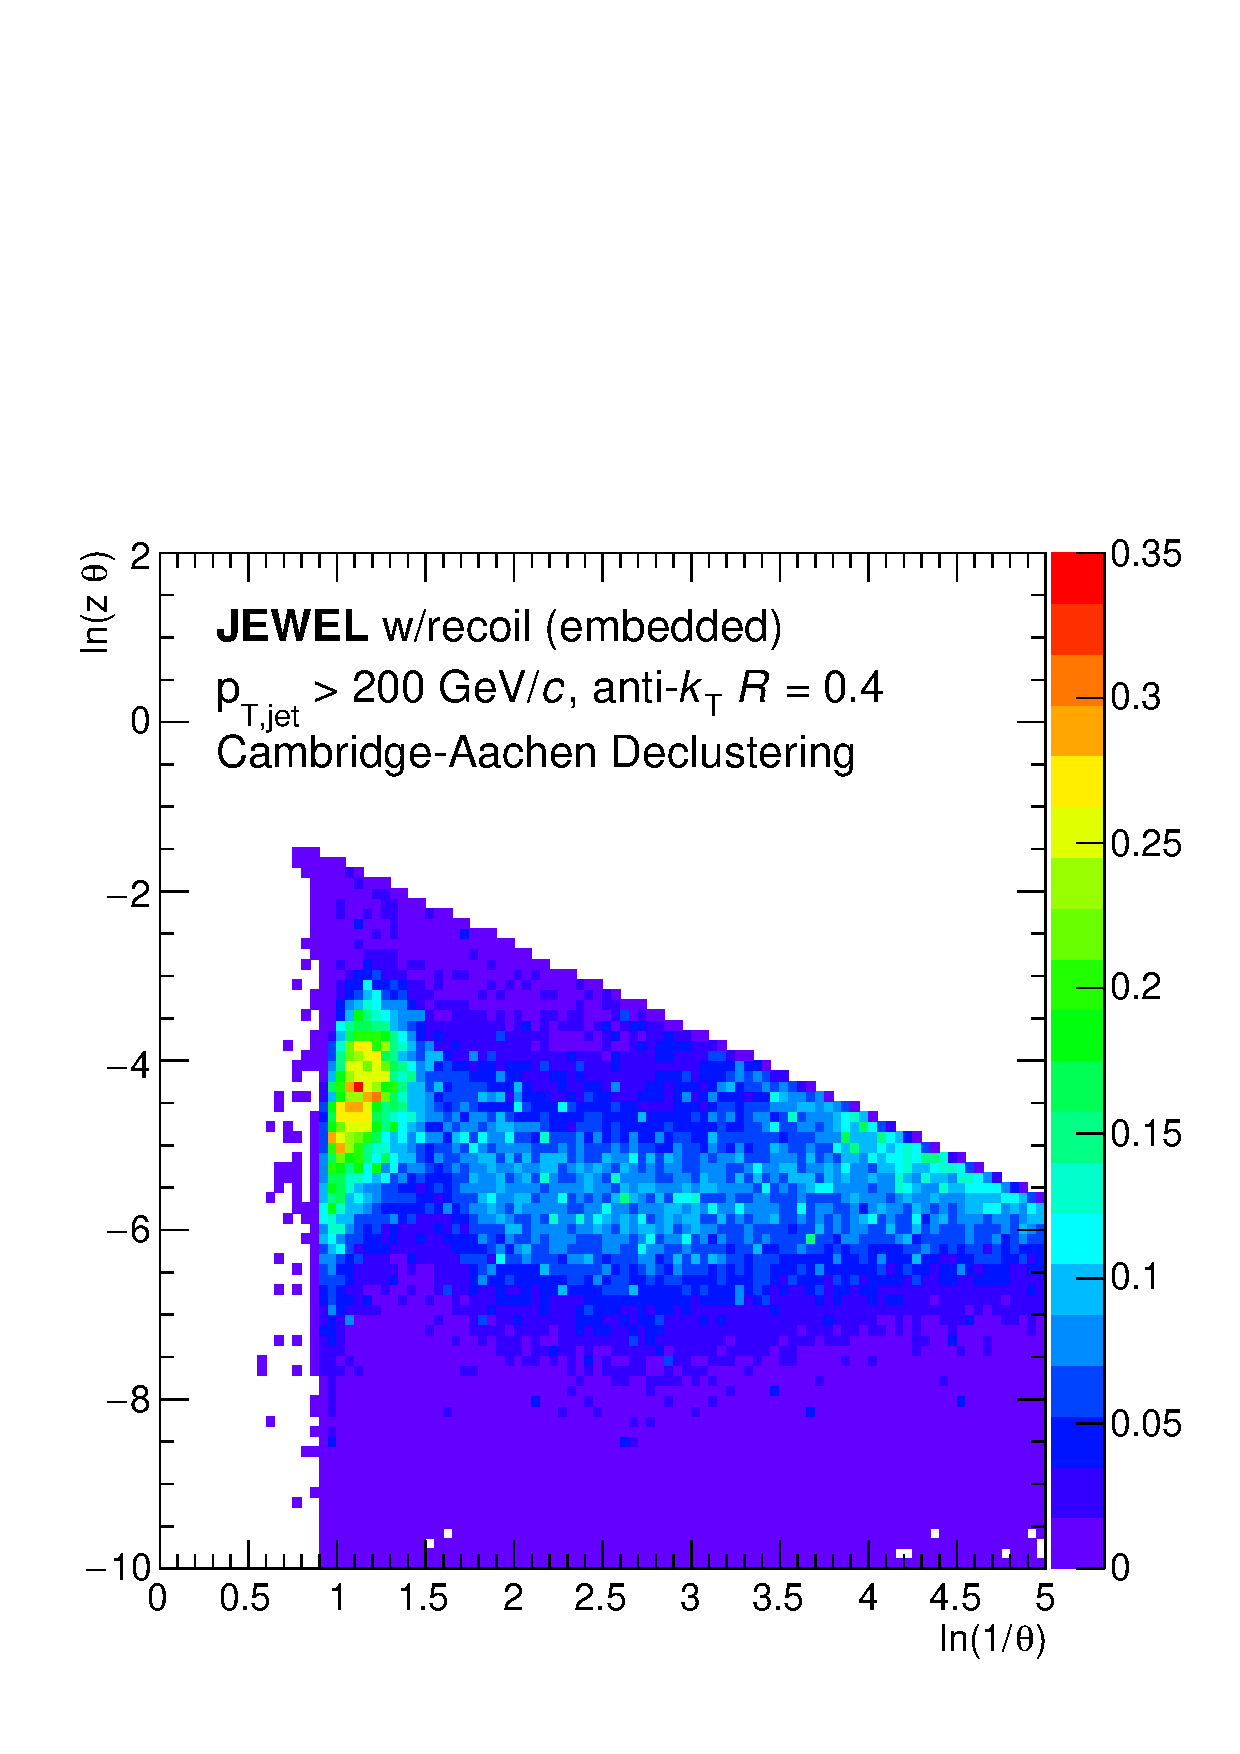
\includegraphics[width=0.32\textwidth]
{figures/LundMC/FinalPlots/Jewel_MedEmb_RecoilOn.pdf}\\
%\includegraphics[width=0.32\textwidth]
%{figures/LundMC/QPythiaEmbeddedDiff}
%\includegraphics[width=0.32\textwidth]
%{figures/LundMC/Jewel_EmbDiff_RecoilOff}
%\includegraphics[width=0.32\textwidth]
%{figures/LundMC/Jewel_EmbDiff_}
\caption{Impact of the uncorrelated background in the splitting map of the medium parton showers QPYTHIA and JEWEL. Upper row shows the resulting splitting map when embedding the modeled showers in a background. 
%Lower row shows the difference of the showers with and without embedding.
\kmt{Point out that there was background subtraction step performed here (Leticia, is it CS of area-based?).}
}
\label{fig:UncorrelatedBkgSignal}
\end{figure}
%%%%%%%%%%%%%%%%%%%%%%%%%%%%%%%%%%%%%%%%
As expected, this a prominent feature for the in-medium showers as well.
Similar plots are shown for QPYTHIA and JEWEL embedded showers are shown in \autoref{fig:UncorrelatedBkgSignal}. The upper row correspond to QPYTHIA, JEWEL ``Recoils Off'' and JEWEL ``Recoils on'' embedded onto a thermal background. 
%The lower plot show the difference of the splitting map before and after embedding. 
Strikingly, all three plots share a similar dominant feature at large angles. This is confirmed by subtracting the generator-level events from the embedded ones. However, we observe that after embedding, the difference to the vacuum reference (also embedded) is still significant, meaning that the differences in the fragmentation pattern from different generators survive the presence of an underlying event, albeit with significant distortions.
